\chapter{Resultados}
\label{sec:results}

Essa seção apresenta os resultados das análises que desenvolvemos sobre os dados
da pesquisa OD 17. Começamos com a exploração dos recursos de visualização
suportados pelo \emph{CUBu}, com ênfase na codificação visual de atributos
densidade, distância e direção das viagens. Esses aspectos são apresentados a
seguir nas Seções~\ref{sec:density},~\ref{sec:trail-overlap},~\ref{sec:length-direction},~and~\ref{sec:coloring}.
Posteriormente, utilizando tais recursos visuais analisamos outros padrões de
mobilidade específicos a subconjuntos dos dados, os quais são detalhados nas
Seções~\ref{sec:strata},~\ref{sec:students},~\ref{sec:peak-hours},~\ref{sec:dist_reasons},~and~\ref{sec:mode}.

\section{Visualizando a densidade dos \emph{bundles}}
\label{sec:density}

Na Seção~\ref{sec:bundling} explicamos como a operação de \emph{bundling}
faz o agrupamento de trajetórias simplificando a visualização e reduzindo a oclusão
da imagem. No entanto, tal operação não nos diz quantas trajetórias foram agrupadas em
um \emph{bundle}. A solução para isso, primeiramente apresentada por \cite{holten06},
é desenhar linhas semi-transparentes, cada uma com uma transparência fixa $\alpha < 1$.
Assim, a combinação mostrará trajetórias de alta densidade como mais opacas e as de baixa
densidade como mais transparentes. Apesar da transparência ajudar na diferenciação
de áreas densas, ela por si só não é uma variável visual quantitativa forte \cite{slocum09}.
Então, codificamos também a densidade das trajetórias em cores, utilizando
os valores estimados pelo KDE durante o processo de \emph{bundling} (ver Seção~\ref{sec:bundling}).
A Figura~\ref{fig:bundled-graph-density}a mostra uma visualização obtida usando codificação
da densidade em cores aplicada em todo o conjunto de dados da OD17 contendo
as \num{685115} viagens. Podemos ver alguns caminhos com maior densidade, mas a imagem
ainda apresenta uma demasiada carga de informação e muitas áreas opacas. Isso ocorre pelo fato de que,
usualmente em GPUS de consumo comum, a transparência $\alpha$ é modelada por um valor
inteiro de 8 bits. Portanto, apenas 255 níveis de transparência diferentes são possíveis,
ou seja, apenas 255 níveis de densidade das trajetórias podem ser exibidos. Valores
de $\alpha$ muito altos saturam o canal de transparência
onde ocorrem as densidades mais altas - todas as densidades acima de 255 são fixadas
em 255. Valores abaixo de 1/255 resultam em nenhuma imagem, uma vez que
isso corresponde a opacidade zero na representação de 8 bits.

Para resolver este problema, mapeamos a densidade $\rho$ de duas maneiras,
transparência e cor. Já que $\rho$ é calculado precisamente como um número
de ponto flutuante durante a estimação do KDE, nenhum valor é truncado ou arredondado.
Essa estimativa da densidade permite modular a transparência para destacar ainda
mais as áreas de alta densidade e reduzir a oclusão da imagem -- uma outra alternativa
seria utilizar valores maiores de kernel $k$, o que agruparia ainda mais as trajetórias, gerando
\emph{bundles} mais fortes, porém também iria causar uma maior distorção das linhas.
A Figura~\ref{fig:bundled-graph-density}b mostra o \emph{bundling} aplicado nos mesmos
dados da Figura~\ref{fig:bundled-graph-density}a. Podemos observar que os \emph{bundles}
aparecem mais salientes após aplicar a modulação da transparência. A imagem sugere que a rede do tráfego metropolitano
pode ser dividida em algumas ramificações principais que são fortemente conectadas à área central,
onde a cidade de São Paulo está localizada. Isso faz sentido considerando que esta é a parte
mais populosa da área metropolitana. Além disso, a maioria dos sistemas de transporte
cruzam o centro da capital, incluindo linhas de metrô, trem, e as principais vias expressas.

\begin{figure}[!htb]
  \centering
  \captionsetup{justification=centering}
  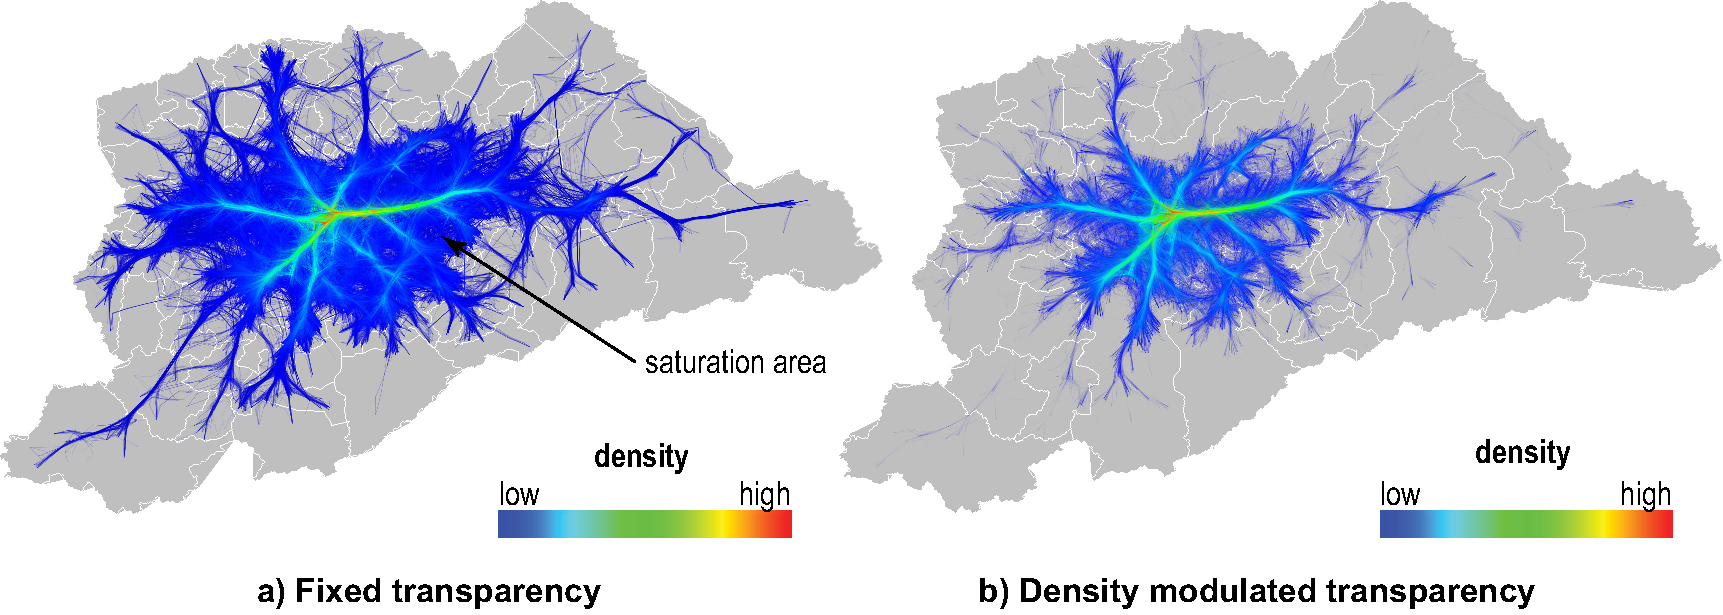
\includegraphics[width=0.98\textwidth]{../figuras/figure1}
  \caption{\emph{Bundling} das trajetórias coloridas pela densidade (a) valores fixos e \\(b) transparência modulada.}
  \label{fig:bundled-graph-density}  
\end{figure}

% % How we calculated 44%:
% %
% % 1. Take all trips that indicate bus, metro, and train as
% %    the main transportation mode -> this is the amount of
% %    trips by public transportation
% %
% % 2. Take all trips that indicate use of metro or train for
% %    some portion of the trip and divide that by the amount
% %    of trips by public transportation
% %
% % Using the tables from pages 46 and 49 of
% % http://www.metro.sp.gov.br/pesquisa-od/arquivos/Ebook%20Pesquisa%20OD%202017_final_240719_versao_4.pdf
% %
% % We consider that:
% % trips using bus as the main transportation mode: 8034
% % trips using train as the main transportation mode: 1245
% % trips using metro as the main transportation mode: 3400
% % total trips by public transportation: 8034 + 1245 + 3400 = 12679
% %
% % trips using metro for some portion of the trip: 3400
% % trips using train for some portion of the trip: 2272
% % total trips involving train or metro: 3400 + 2272 = 5672
% %
% % Percentage = 5672*100/12679 = 44.73%
% %
% % Not relevant for the text, just a curiosity:
% % the percentage in relation to all motorized trips is 5672*100/28280=20.05%

\section{Infraestrutura de metrô e trem \emph{vs} \emph{bundling}}
\label{sec:trail-overlap}

O sistema de transporte público é o mais utilizado pelos moradores da RMSP. O
impacto da malha ferroviária sobre o deslocamento de pessoas fica claro quando
desenhamos as linhas ferroviárias ao longo das trajetórias agrupadas com o
\emph{bundling}. A Figura~\ref{fig:rails} mostra a alta correspondência dos
\emph{bundles} com os caminhos das linhas ferroviárias (desenhadas em preto).
Tendo em vista que, de acordo com a pesquisa OD17, cerca de 44\% das viagens
diárias de transporte público envolvem metrô ou trens, este é um resultado
esperado. Curiosamente pode-se questionar se o sistema ferroviário foi planejado
com precisão para atender a demanda, como sugere a visualização agrupada, ou se
a disponibilidade dessa opção de transporte influenciou a existência de fluxos
tão densos. Embora não temos os insumos para responder a essa pergunta, os
gestores de tráfego podem usar esse tipo de visualização para elaborar políticas
para o transporte público. Apesar de não expressar nenhuma grande surpresa sobre os
dados analisados, este é um resultado bastante importante, pois consideramos que a alta
correlação entre o \emph{bundling} das trajetórias e as linhas das ferrovias
também indica boas configurações de parâmetros para esse tipo de visualização na
escala da região metropolitana.

Ressaltamos que que este tipo de correlação (de \emph{bundles} com estradas) não
é o mesmo que o utilizado no método RAEB, \cite{zeng:19}. No método RAEB, o
agrupamento foi feito explicitamente para seguir estradas. Em nosso caso, as
linhas são sobrepostas sobre \emph{bundles}, que foram gerados unicamente a partir dos
dados da OD. Pode-se argumentar que RAEB, neste sentido, produz \emph{bundles}
mais ``corretos'', uma vez que estes são forçados para seguir as estradas. No
entanto, olhando mais de perto, podemos ver que RAEB não pode ter todos os
\emph{bundles} seguindo precisamente todos os caminhos das estradas - pois isso
basicamente bloquearia qualquer agrupamento do \emph{bundling} e resultaria no próprio
mapa das estradas. Além disso, RAEB requer que o registro dos pontos das trajetórias
seja feito dentro de uma rede rodoviária precisa. Isso torna-o
significativamente mais complexo para implementar e mais caro para processar do
que nossa solução baseada em \emph{CUBu}.

\begin{figure}[!htb]
  \centering
  \captionsetup{justification=centering}
  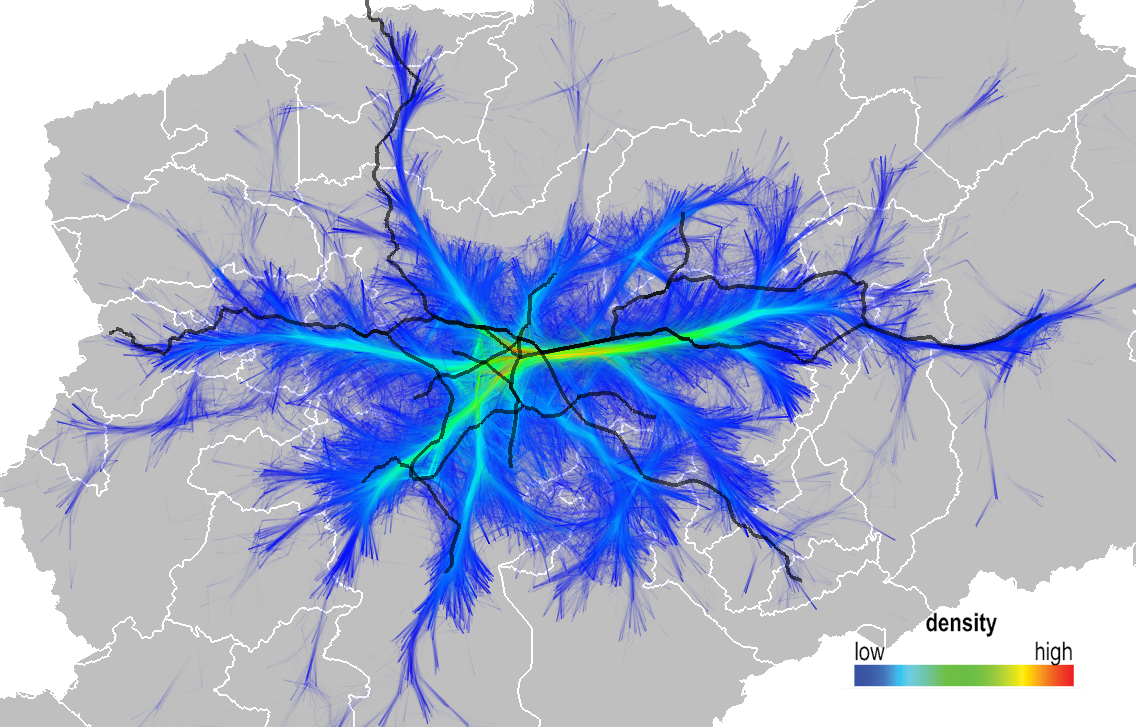
\includegraphics[width=0.98\textwidth]{../figuras/rail-lines.png}
    \caption{\emph{Bundling} das trajetórias coloridas pela densidade e a malha ferroviária da RMSP}
  \label{fig:rails}  
\end{figure}

\section{Mapeando distância e direção no \emph{bundling}}
\label{sec:length-direction}

Para explorar a mobilidade urbana por diferentes perspectivas, precisamos de
meios para visualizar os múltiplos atributos dos dados. Dois
importantes atributos para o estudo de padrões de mobilidade são distância
percorrida na viagem e a sua direção. As Figuras~\ref{fig:attributes-length} e
\ref{fig:attributes-direction} mostram a visualização de todo o conjunto de
dados OD17 mapeando a distância e direção, respectivamente.

Na Figura~\ref{fig:attributes-length} codificamos nas cores os comprimentos das
viagens. Nela utilizamos o mesmo mapa de cores (arco-íris) da
Figura~\ref{fig:rails}, além também de aplicar a modulação da transparência por densidade,
conforme explicado na Seção~\ref{sec:density}. Nesta imagem, podemos observar
uma única curva vermelha aparentemente na horizontal. Sua alta opacidade implica
que há muitas viagens longas, todas mapeadas perfeitamente para essa trajetória
entre a mesma origem e destino (se não o fizessem, veríamos um \emph{bundle} se
ramificando no formato de um leque em vez de uma curva precisa). Esta é uma
descoberta interessante que, argumentamos, não poderia ser facilmente encontrada
usando métodos não visuais. Apesar desse ponto fora do comum, as outras trajetórias,
em geral, percorrem distâncias regulares. \emph{Bundles} de longa distância como
este podem indicar falta de serviços ou recursos que não satisfazem as regiões
locais, obrigando as pessoas a percorrerem longas distâncias para acessá-los. A
pesquisa OD17 contém mais informações que podem ajudar a investigar o motivo
dessas longas viagens.

A Figura~\ref{fig:attributes-direction} mostra os mesmos dados da
Figura~\ref{fig:attributes-length}, mas ao invés da distância são as direções
das viagens que estão codificadas em cores. Para este atributo em específico,
usamos ainda um recurso do \emph{CUBu}, que separa trilhas em direções opostas
em dois \emph{bundles} quase paralelos. Podemos ver claramente a existência de
trajetórias paralelas ao longo dos \emph{bundles}, o que não é surpreendente
porque a pesquisa OD registra o trajeto típico das pessoas que inclui os
deslocamentos de ida e vinda de volta para suas origens. No entanto, essa
simetria das trajetórias possivelmente não seria observada se analisássemos um
curto período do dia.

\begin{figure}[!htb] \centering \captionsetup{justification=centering}
  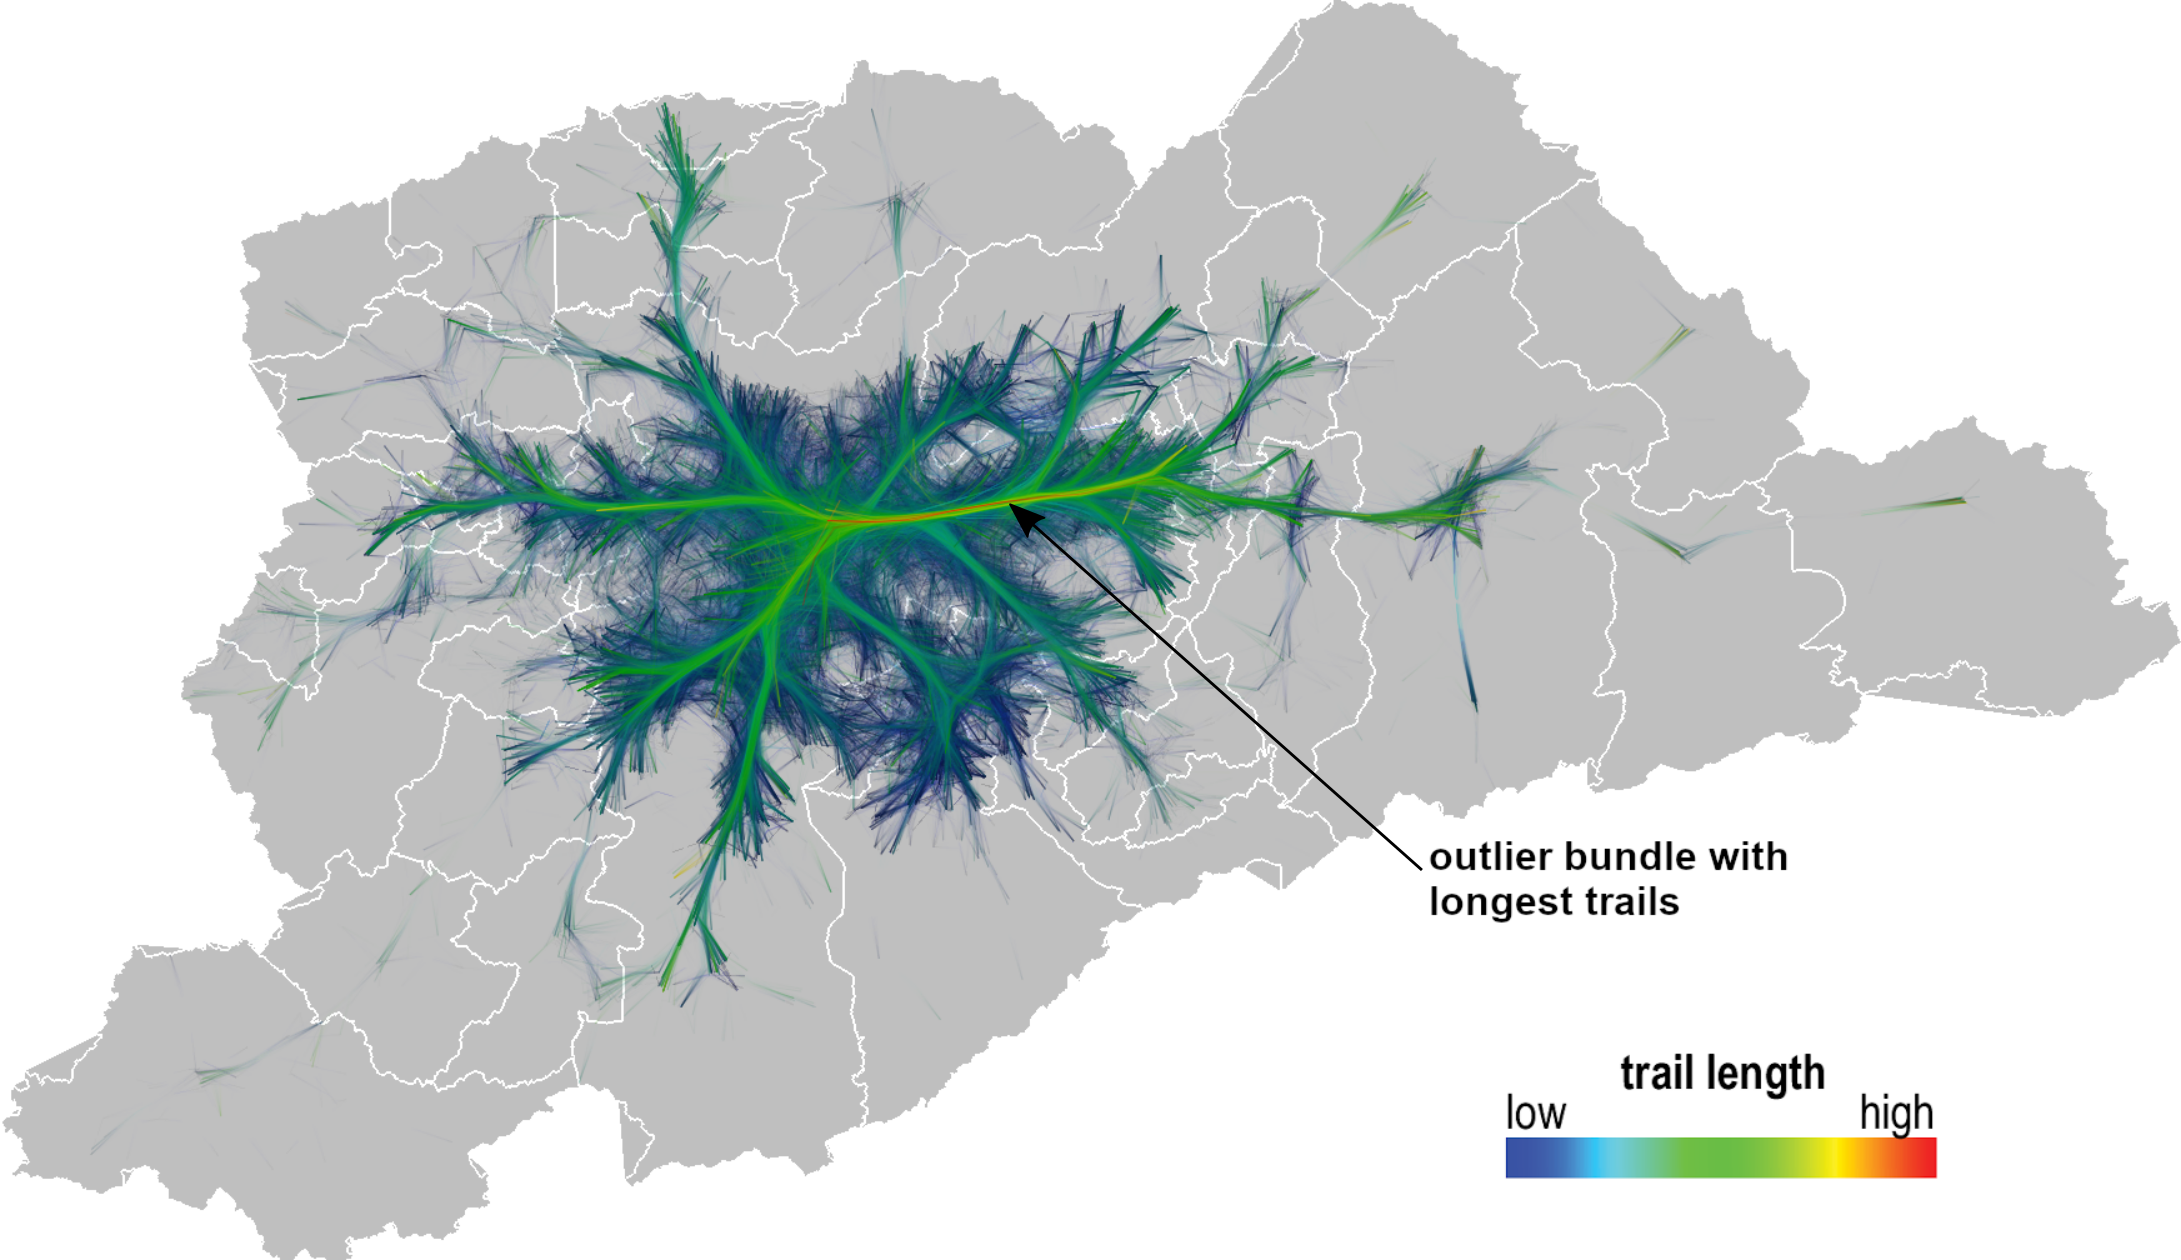
\includegraphics[width=0.98\textwidth]{../figuras/distances.png}
  \caption{Mapeamento da distância das viagens em cores. \label{fig:attributes-length}}
  \end{figure}

\begin{figure}[!htb]
  \centering
  \captionsetup{justification=centering}
  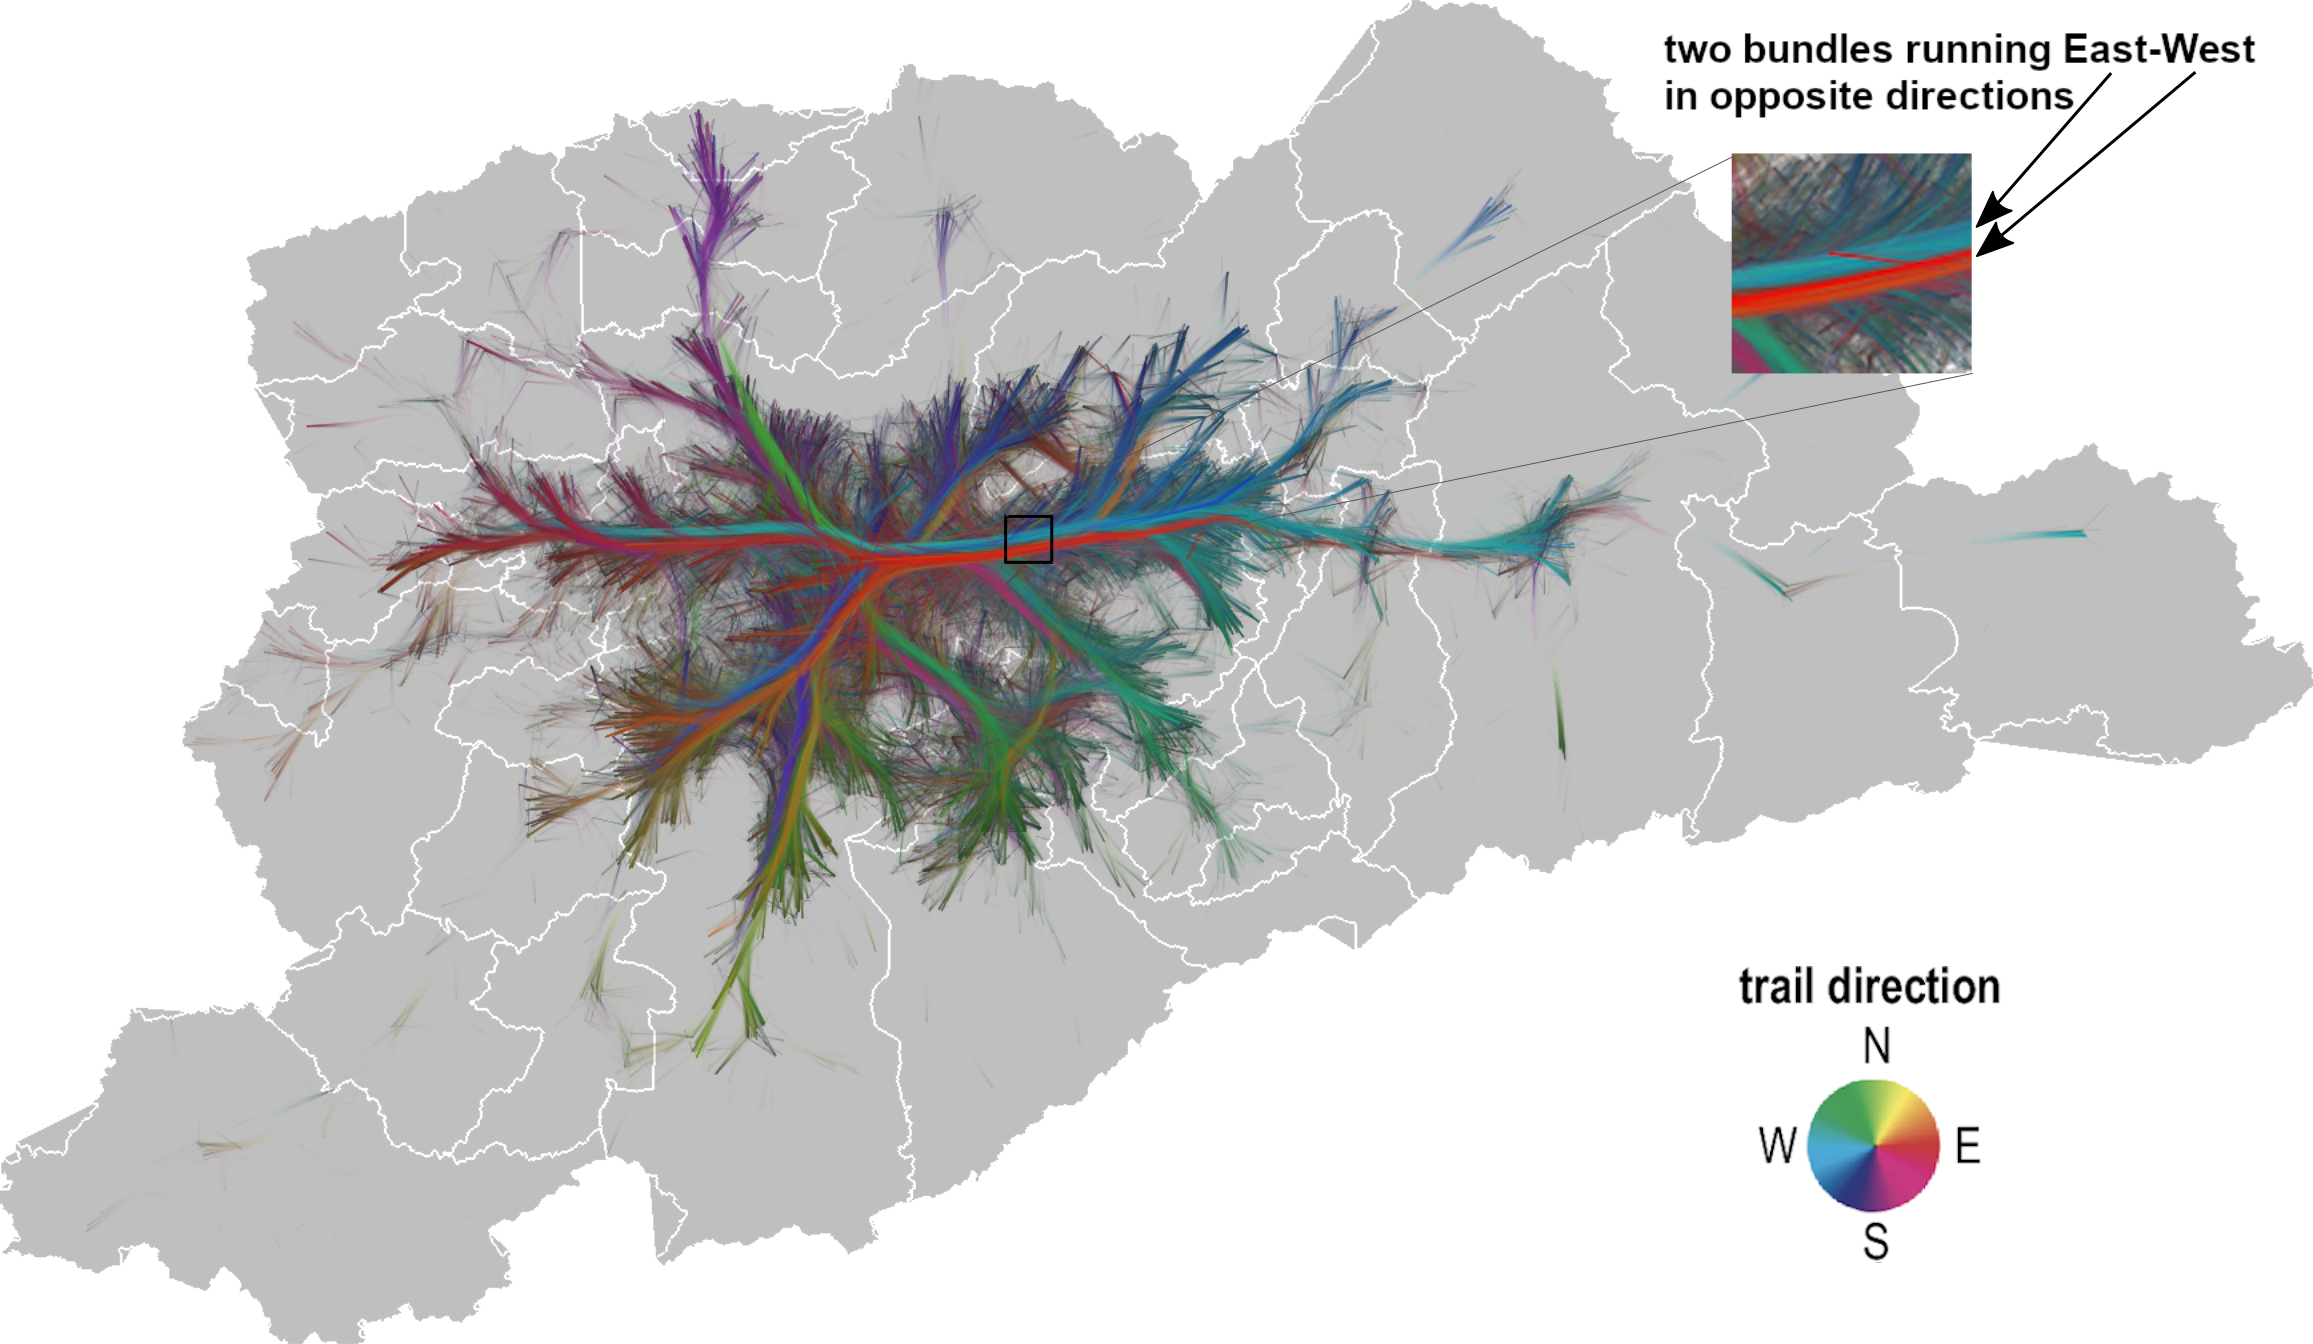
\includegraphics[width=0.98\textwidth]{../figuras/directions.png}
  \caption{Mapeamento da direção das viagens em cores. \label{fig:attributes-direction}}
\end{figure}

\section{Visualização dos modos de transporte: ônibus locais \emph{vs} intermunicipais}
\label{sec:coloring}

Como mostramos na Seção~\ref{sec:pesquisa-od}, o conjunto de dados OD17 contém
17 modos de transporte. Embora fosse ideal ser capaz de ver as 17 categorias ao
mesmo tempo em nossa visualização com \emph{bundling}, isso não seria fácil de
se obter, uma vez que exigiria a codificação simultânea de 17 diferentes
categorias de transporte. Então, nós utilizamos a transparência para esconder
trajetórias de acordo com seletores que podem ser configurados na interface para
filtrar as trajetórias pelo modo de transporte. A
Figura~\ref{fig:bus-integration} mostra como nos aplicamos tais filtros para
visualizar a integração entre os ônibus da cidade de São Paulo (ônibus locais) e
os ônibus intermunicipais. As trajetórias originais e agrupadas com \emph{bundling}
são apresentadas lado a lado. Cada meio de transporte tem uma coloração distinta -
oliva para ônibus locais e azul para ônibus intermunicipais.

Podemos ver mais claramente na Figura~\ref{fig:bus-integration-zoom} que esses diferentes sistemas
de transporte parecem se complementar. A cidade de São Paulo tem um comércio e
uma indústria muito ativa, que recebe muitos trabalhadores advindos das cidades
vizinhas. Assim, a disponibilidade de transporte público e sua integração é
muito importante para essas pessoas. Esse tipo de filtragem juntamente com as
técnicas de \emph{bundling} ajudam a entender melhor as correlações entre os
atributos dos dados - neste caso, modos de transporte.

\begin{figure}[!htb]
  %\centering
  %\raggedright\noindent\hspace{-\margemesq}\hspace{.01\paperwidth}%
  %\begin{subfigure}{0.49\paperwidth}
  \raggedright\noindent\hspace{-.02\textwidth}%
  \begin{subfigure}{0.55\textwidth}
    \centering
    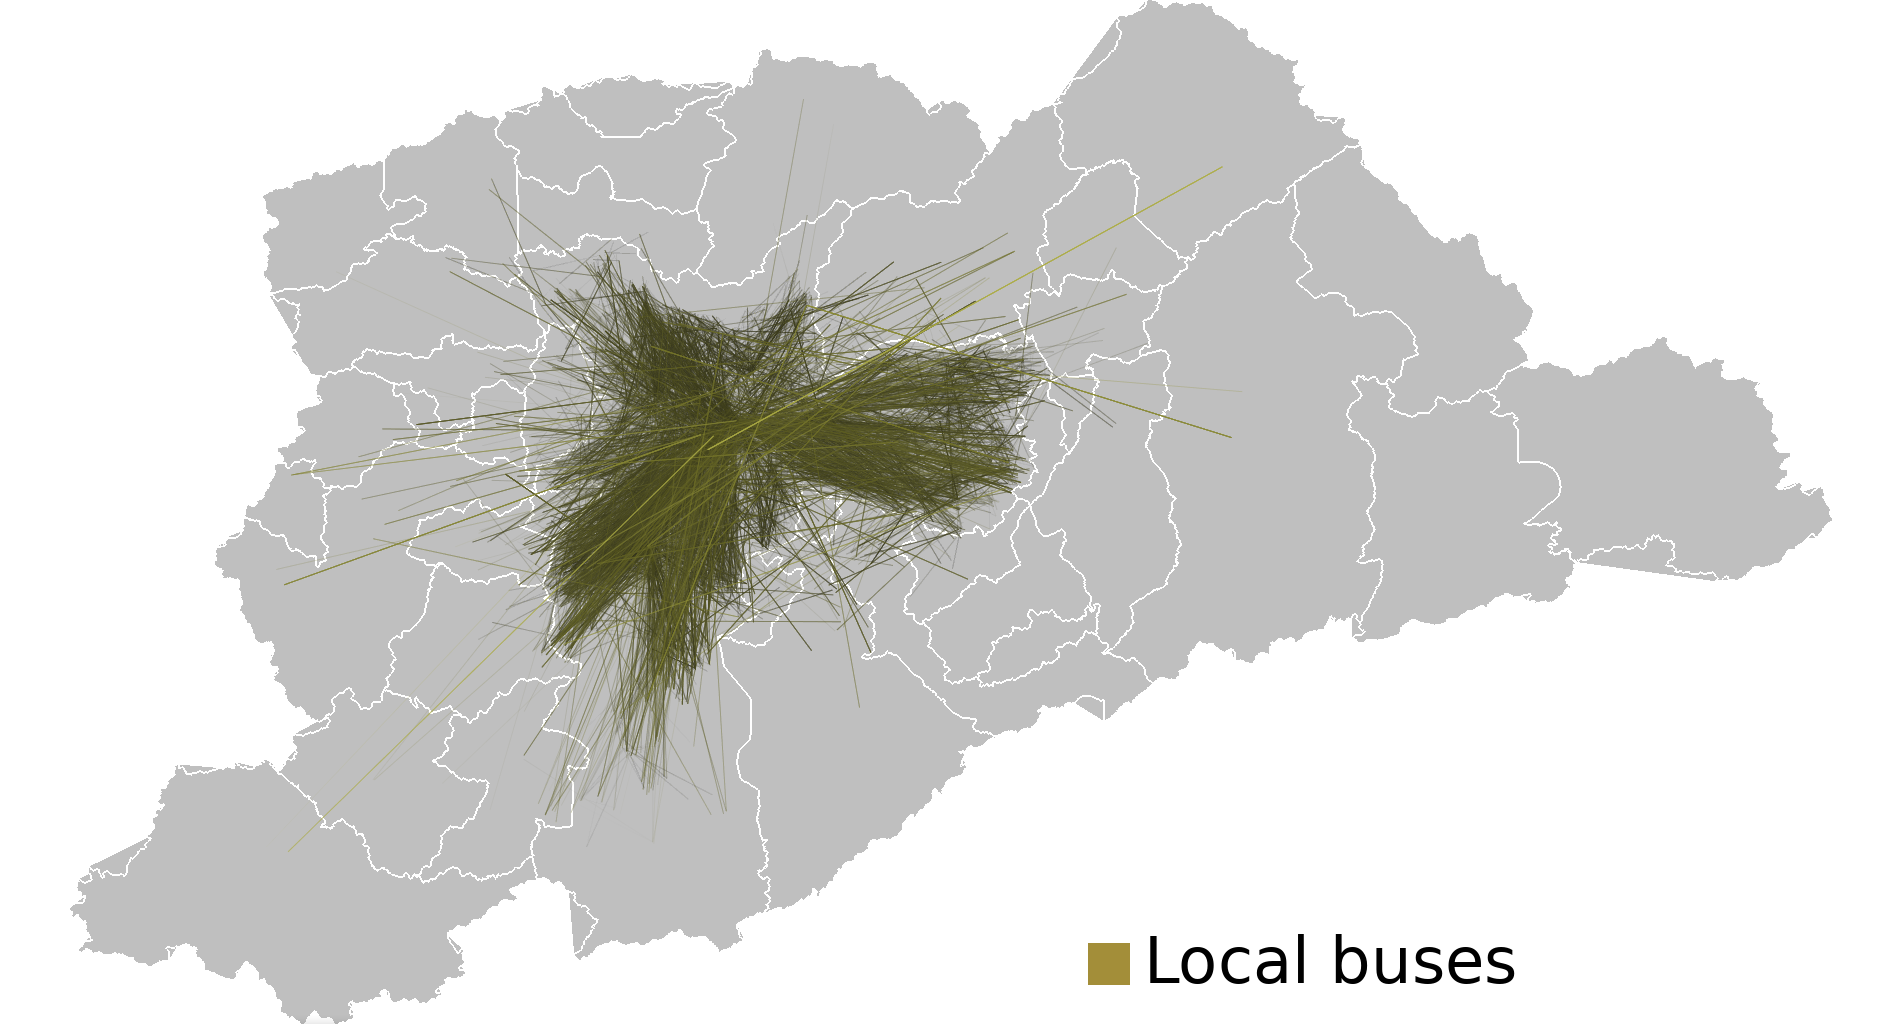
\includegraphics[width=1\textwidth]{../figuras/busesLocalXmetropolitan/unbundled-buses.png}
    \caption{\label{fig:bus-integration-a}}
  \end{subfigure}\nobreak%
  %\begin{subfigure}{0.49\paperwidth}
  \hspace{-.06\textwidth}\nobreak%
  \begin{subfigure}{0.55\textwidth}
    \centering
    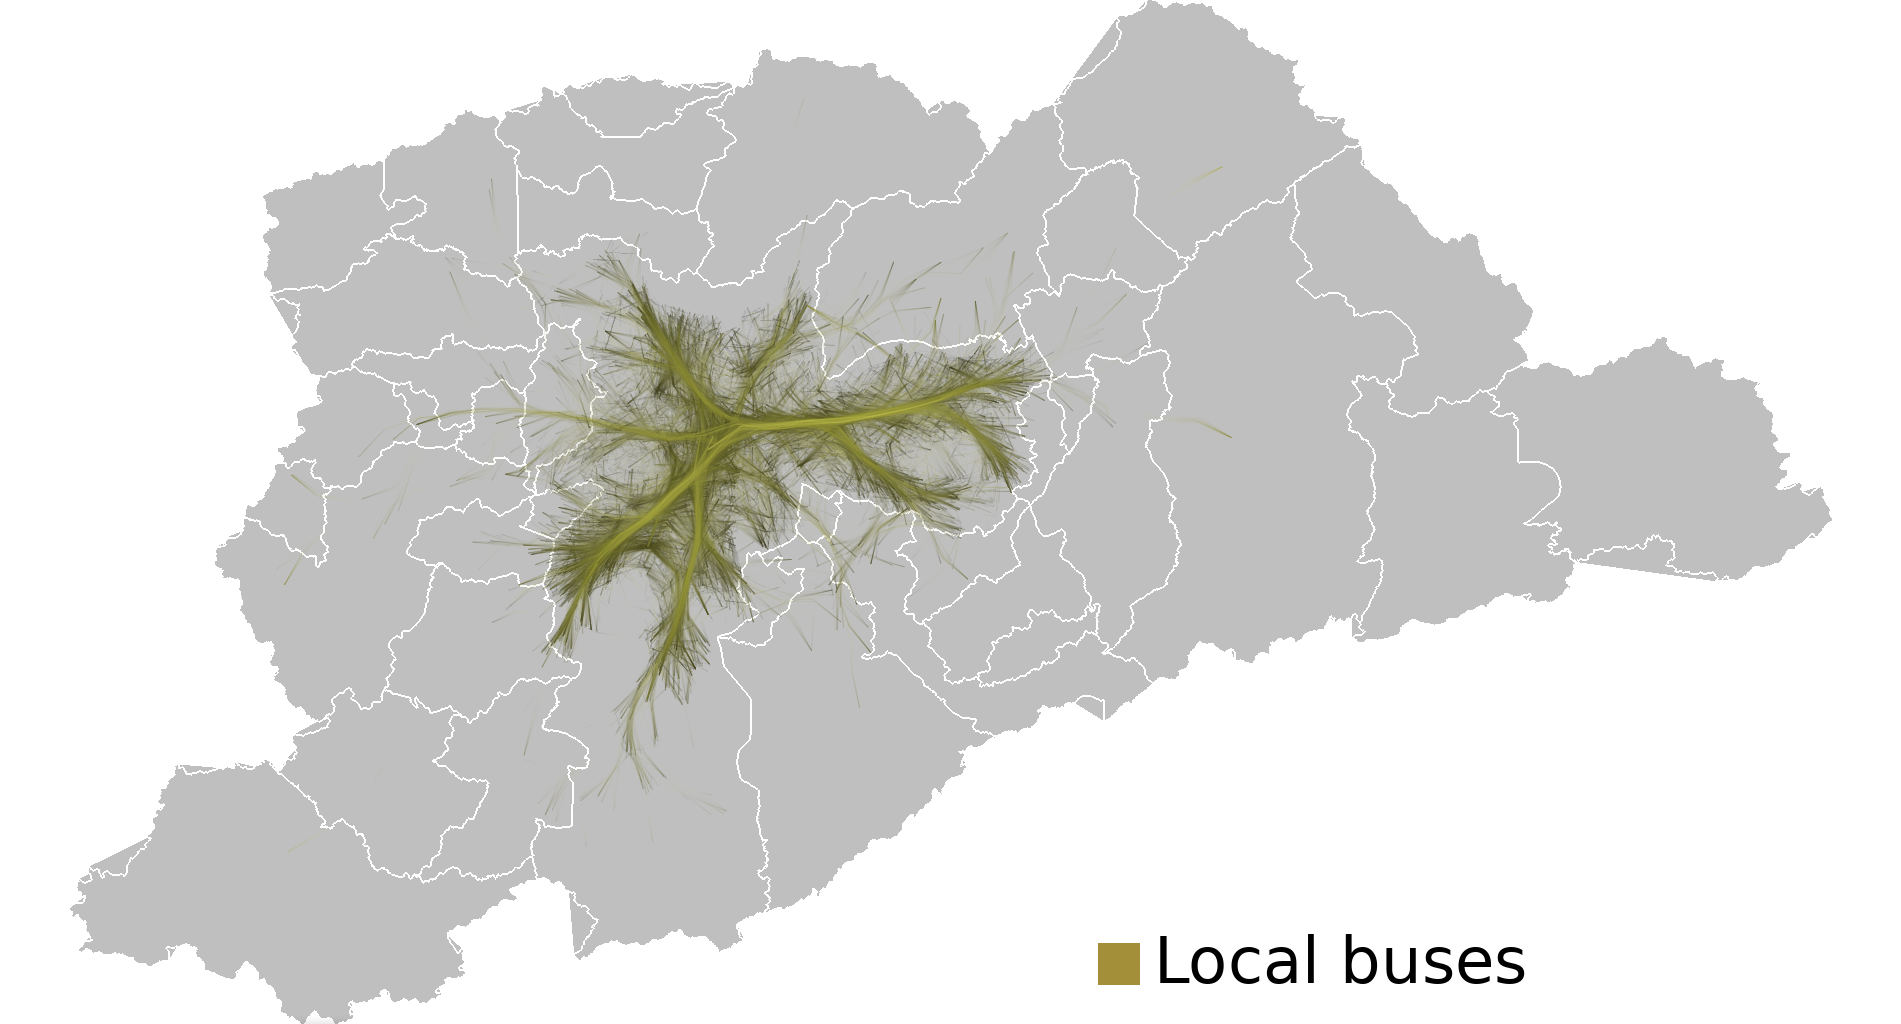
\includegraphics[width=1\textwidth]{../figuras/busesLocalXmetropolitan/bundled-buses-length.png}
    \caption{\label{fig:bus-integration-b}}
  \end{subfigure}

  %\noindent\hspace{-\margemesq}\hspace{.01\paperwidth}\begin{subfigure}{0.49\paperwidth}
  \raggedright\noindent\hspace{-.02\textwidth}%
  \begin{subfigure}{0.55\textwidth}
    \centering
    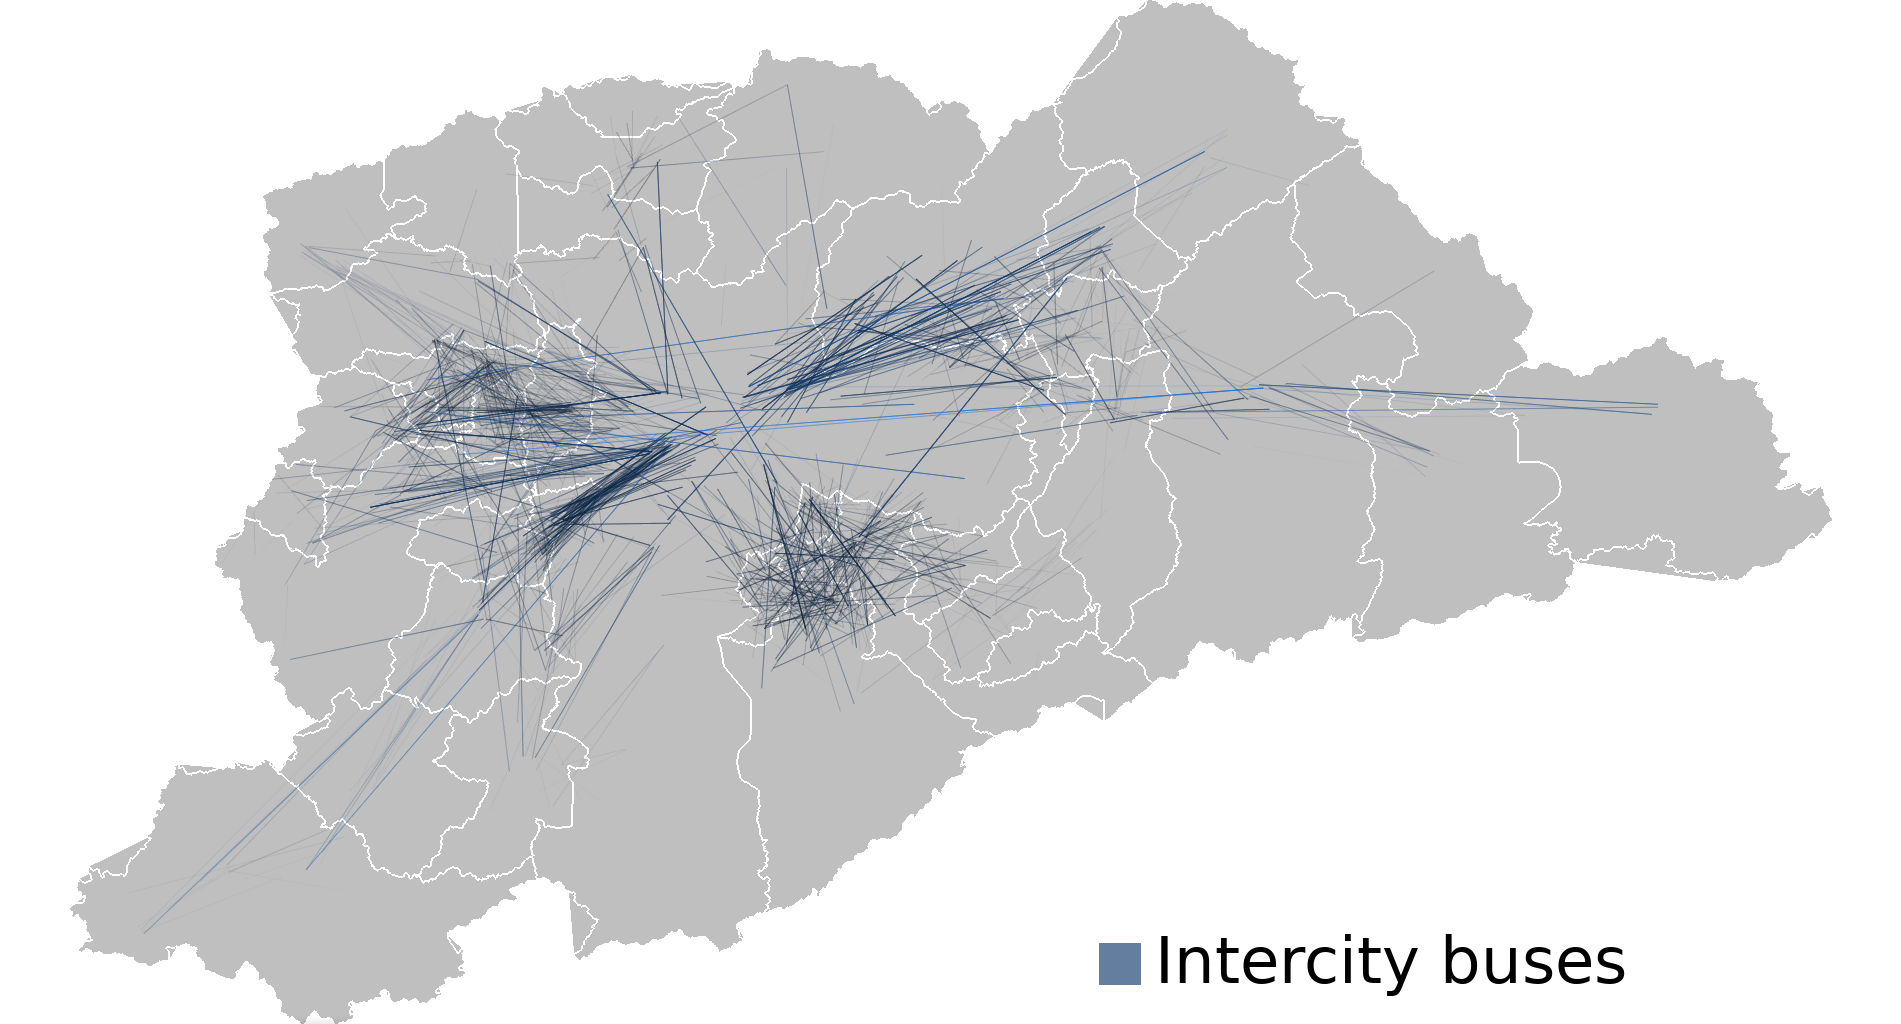
\includegraphics[width=1\textwidth]{../figuras/busesLocalXmetropolitan/unbundled-metropolitan-buses.png}
    \caption{\label{fig:bus-integration-c}}
  \end{subfigure}\nobreak%
  \hspace{-.06\textwidth}\nobreak%
  \begin{subfigure}{0.55\textwidth}
  %\begin{subfigure}{0.49\paperwidth}
    \centering
    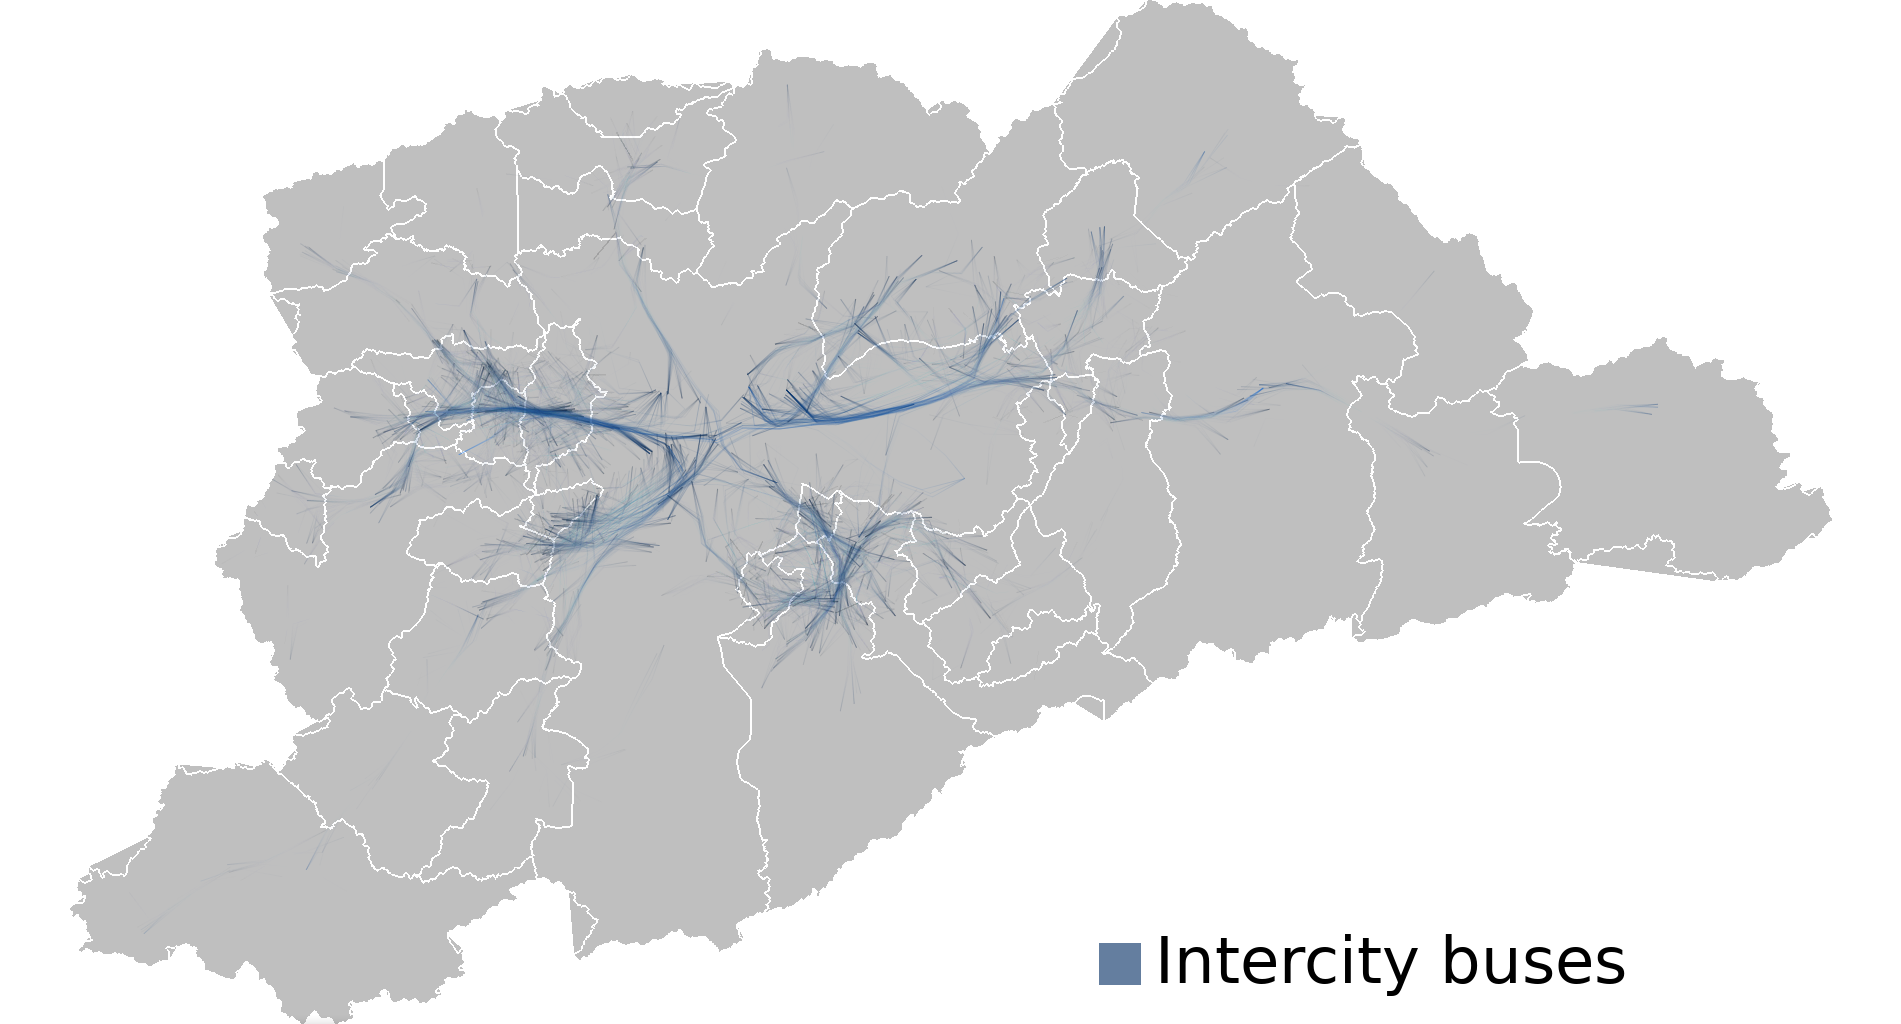
\includegraphics[width=1\textwidth]{../figuras/busesLocalXmetropolitan/bundled-metropolitan-buses-length.png}
    \caption{ \label{fig:bus-integration-d}}
  \end{subfigure}

  %\noindent\hspace{-\margemesq}\hspace{.01\paperwidth}\begin{subfigure}{0.49\paperwidth}
  \raggedright\noindent\hspace{-.02\textwidth}%
  \begin{subfigure}{0.55\textwidth}
    \centering
    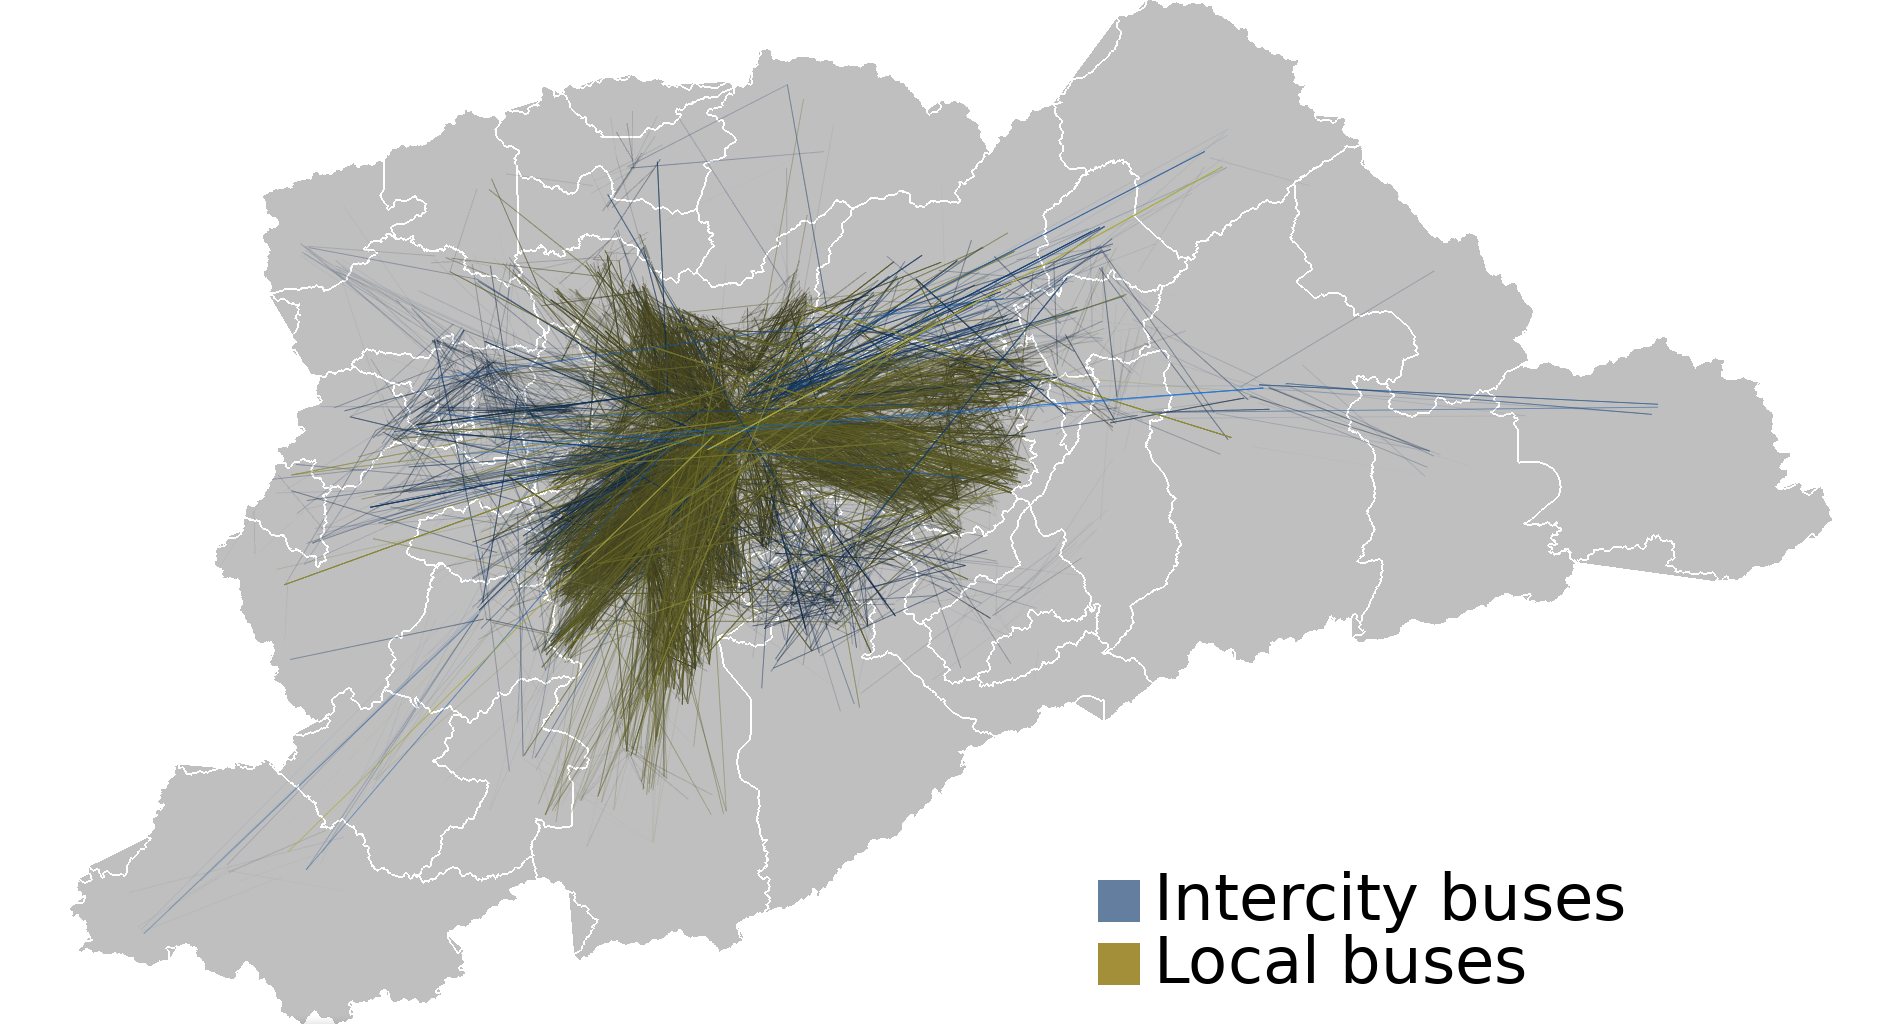
\includegraphics[width=1\textwidth]{../figuras/busesLocalXmetropolitan/unbundled-buses-and-metropolitan.png}
    \caption{\label{fig:bus-integration-e}}
  \end{subfigure}\nobreak%
  \hspace{-.06\textwidth}\nobreak%
  \begin{subfigure}{0.55\textwidth}
  %\begin{subfigure}{0.49\paperwidth}
    \centering
    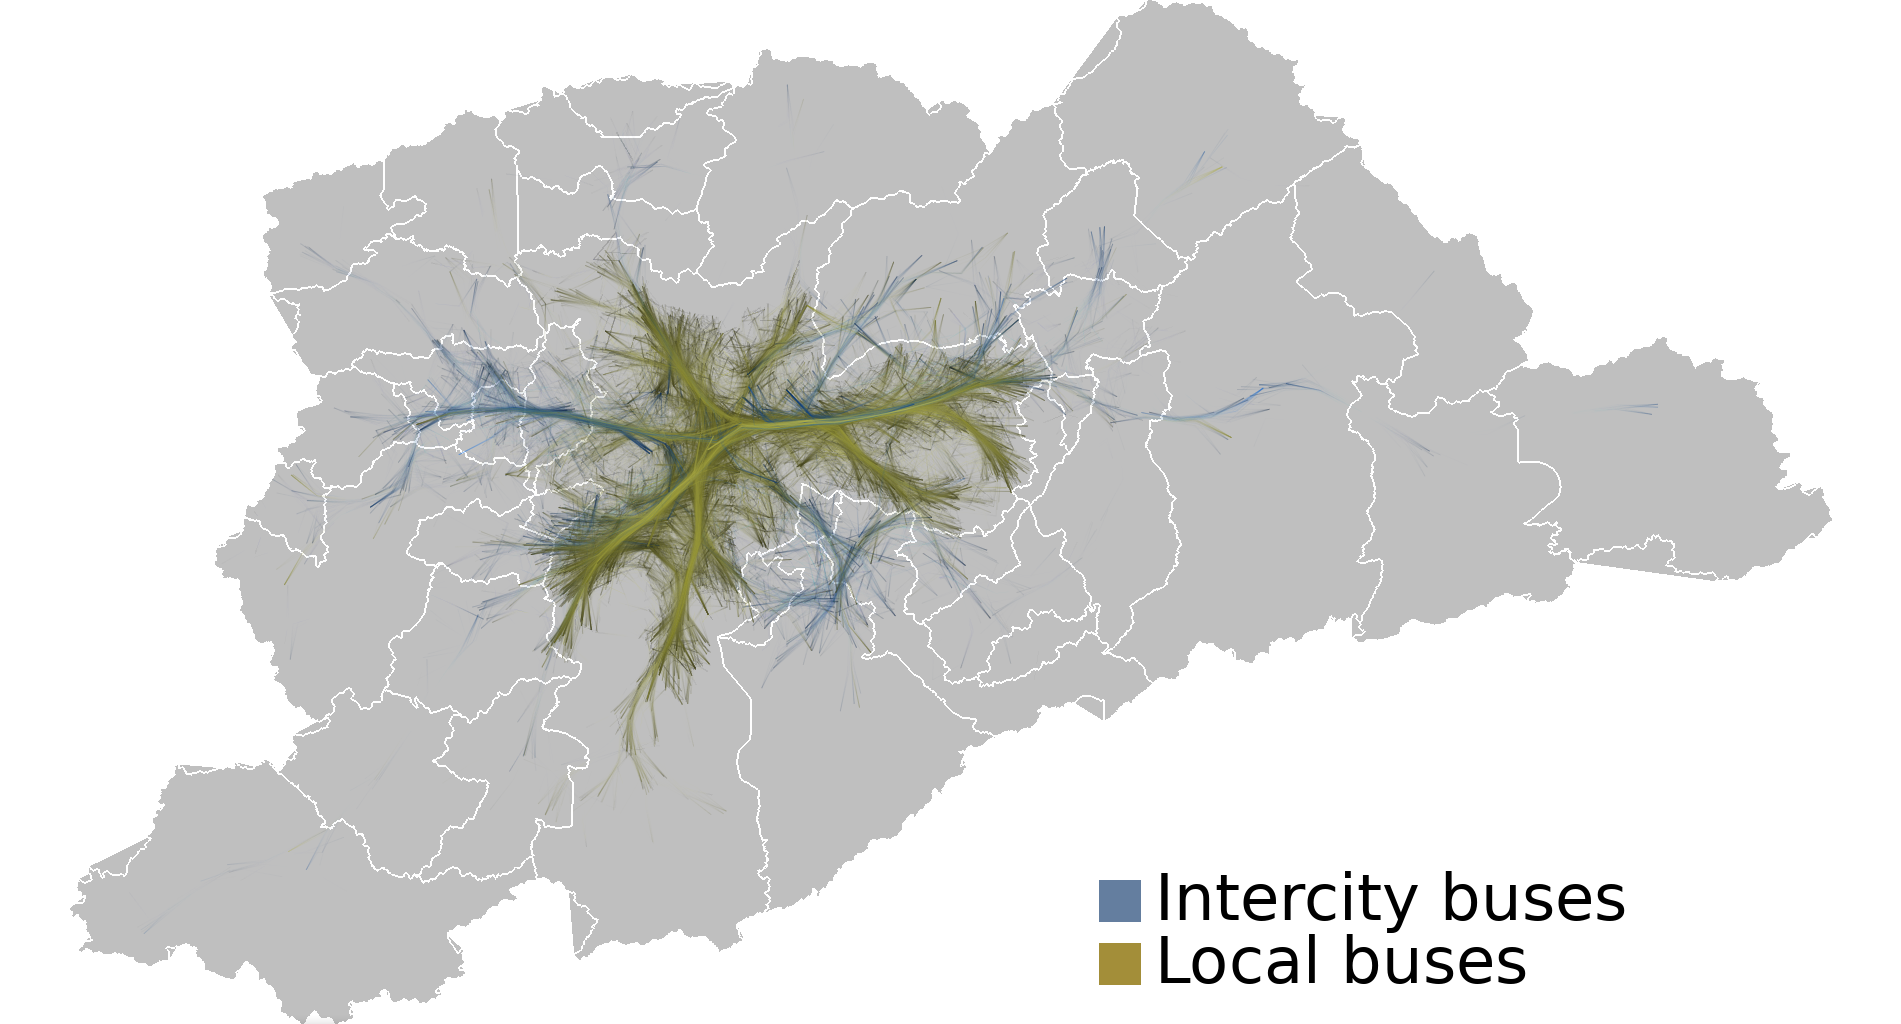
\includegraphics[width=1\textwidth]{../figuras/busesLocalXmetropolitan/bundled-buses-and-metropolitan-length.png}
    \caption{\label{fig:bus-integration-f}}
  \end{subfigure}
  \caption{Viagens filtradas pelo modo de transporte: ônibus locais e intermunicipais. Dados originais à esquerda (a, c, e)  e \emph{bundling} à direita (b, d, f). \label{fig:bus-integration}}
\end{figure}

\begin{figure}[!htb]
  \centering
  \captionsetup{justification=centering}
  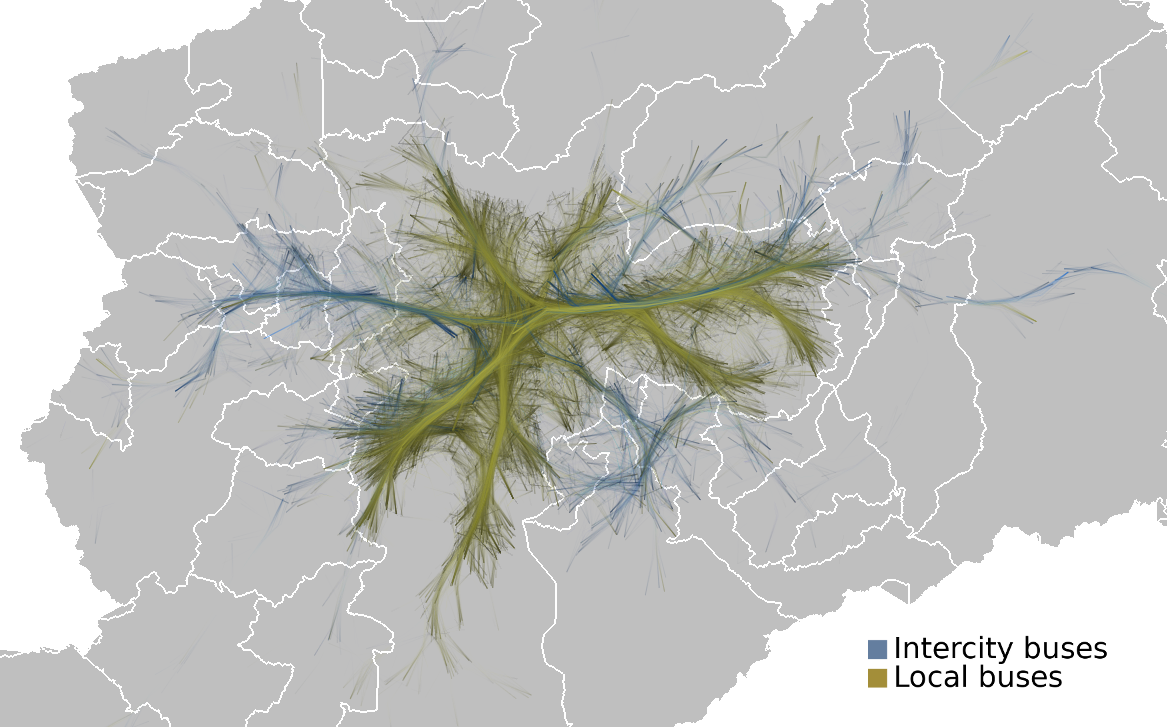
\includegraphics[width=0.98\textwidth]{../figuras/local-intercity-buses}
  \caption{Viagens filtradas pelo modo de transporte: ônibus locais e intermunicipais (ZOOM). \label{fig:bus-integration-zoom}}
\end{figure}

\section{Visualização das diferentes classes sociais}
\label{sec:strata}

Usamos nossa visualização com \emph{bundling} para estudar como os cidadãos com diferentes
condições econômicas se deslocam na RMSP. O Critério de Classificação Econômica
Brasileira (CCEB), \cite{cceb2008} é o índice socioeconômico oficial utilizado no Censo
Demográfico Brasileiro, realizado pelo Instituto Brasileiro de Geografia e
Estatística (IBGE). Ele mede o poder de compra da sociedade brasileira. O CCEB é
dividido em seis níveis ou estratos (Tabela~\ref{tab:becc}). Este índice é usado na pesquisa
OD17 para complementar os dados de mobilidade. A Tabela~\ref{tab:becc} também mostra a renda
média mensal (em reais), e o número de viagens na RMSP para cada nível do CCEB considerando toda a população e apenas
os cidadãos com idade entre 6 e 18 anos que se deslocam para fins de estudos (consulte a
Seção~\ref{sec:students}).

\begin{table}[!htb]
  \small
  \newcommand{\hdr}[1]{\bfseries#1}
  \centering
  \caption{Viagens agrupadas pelo índice CCEB income level, social stratum, and traveler age.\label{tab:becc}}
  \begin{tabular}{>{\footnotesize}c>{\footnotesize}r>{\footnotesize}r>{\footnotesize}r>{\footnotesize}r}
    \toprule
    \multirow{2}[2]{*}{\hdr{Nível CCEB}} & \hdr{Renda mensal} & \hdr{Viagens} & \hdr{Viagens de estudantes}\\
    & \hdr{em reais (R\$)} & \hdr{totais} & \hdr{entre 6 e 18 anos}\\
    \midrule
    A   & 23,345    & 3,062,892  &   184,772\\
    B1  & 10,386    & 3,854,040  &   260,652\\
    B2  & 5,363     & 12,856,182 &   963,242\\
    C1  & 2,965     & 11,277,159 &   976,745\\
    C2  & 1,691     & 7,852,806  &   721,218\\
    D-E & 708       & 2,233,801  &   219,612\\
    \bottomrule
  \end{tabular}
\end{table}

Para comparar os padrões de mobilidade de diferentes estratos sociais CCEB,
aplicamos \emph{bundling} nas viagens de cada estrato separadamente, como
mostrado nas Figuras~\ref{fig:becc-axd-e}~até~\ref{fig:becc-d-e}. Observamos
diferenças significativas nos padrões de mobilidade entre os níveis de renda
mais altos e mais baixos, como mostra a Figura~\ref{fig:becc-axd-e}. O nível $A$
Figuras~\ref{fig:becc-a} apresenta alta densidade no centro da RMSP, que inclui
o entorno do centro da capital. A maior densidade está localizada nos bairros
oeste, sudoeste e nordeste próximos ao centro. Existem fluxos de densidade entre
a capital e as cidades de Barueri e Cotia, que possuem áreas residenciais de
alta renda. Existem outros fluxos de alta densidade ligando a capital às cidades
de São Bernardo do Campo e Santo André. Comparando A ao nível D-E (Figura 18),
vemos que D-E tem os fluxos densos mais elevados na região leste da capital. No
mapa de níveis D-E, podemos ver a ausência de fluxos de alta densidade nas
regiões mais próximas do centro da capital; em contraste, eles estão presentes
no mapa de nível A.

\begin{figure}[!htb]
  \centering
  \captionsetup{justification=centering}
  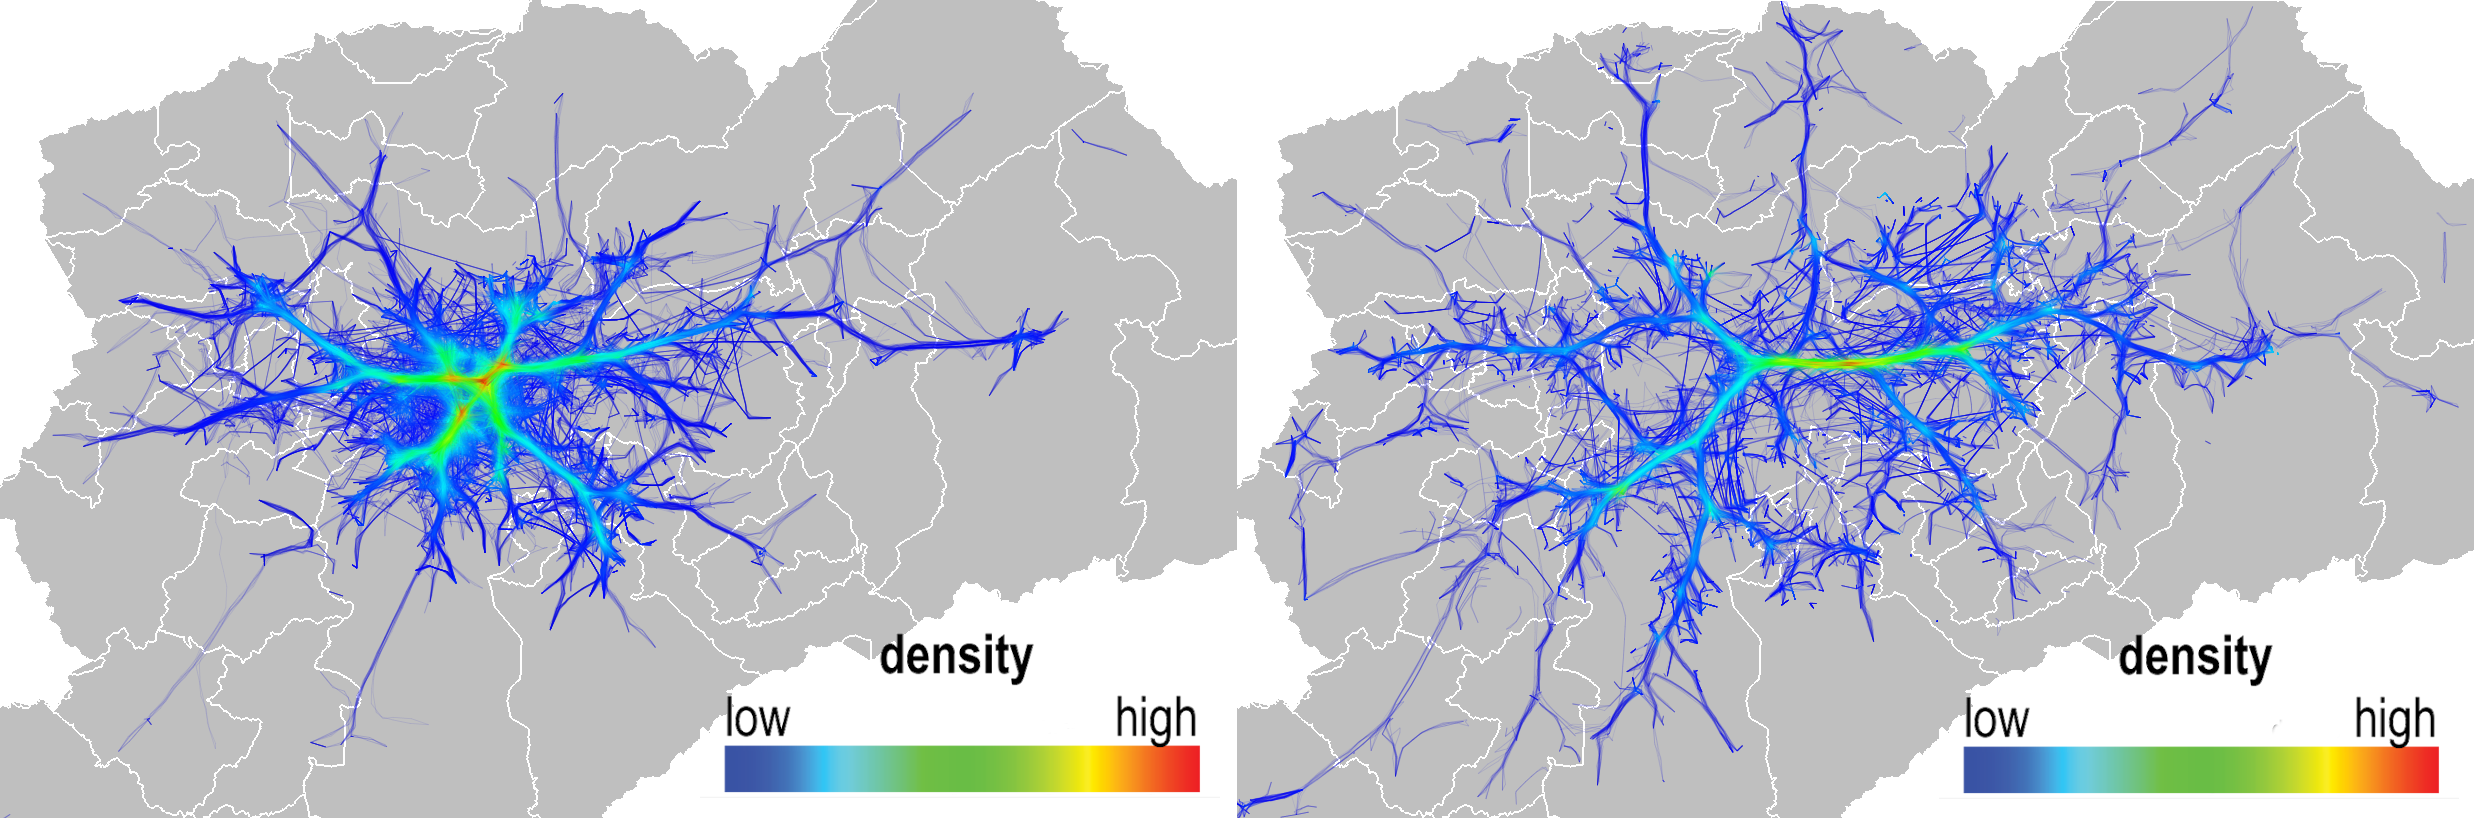
\includegraphics[width=0.98\textwidth]{../figuras/comparison-axd-e-strata-leg.png}
  \caption{Densidade das viagens da classe $A$ (esquerda) e $D$-$E$ (direta). \label{fig:becc-axd-e}}
\end{figure}

\begin{figure}[!htb]
  \centering
  \captionsetup{justification=centering}
  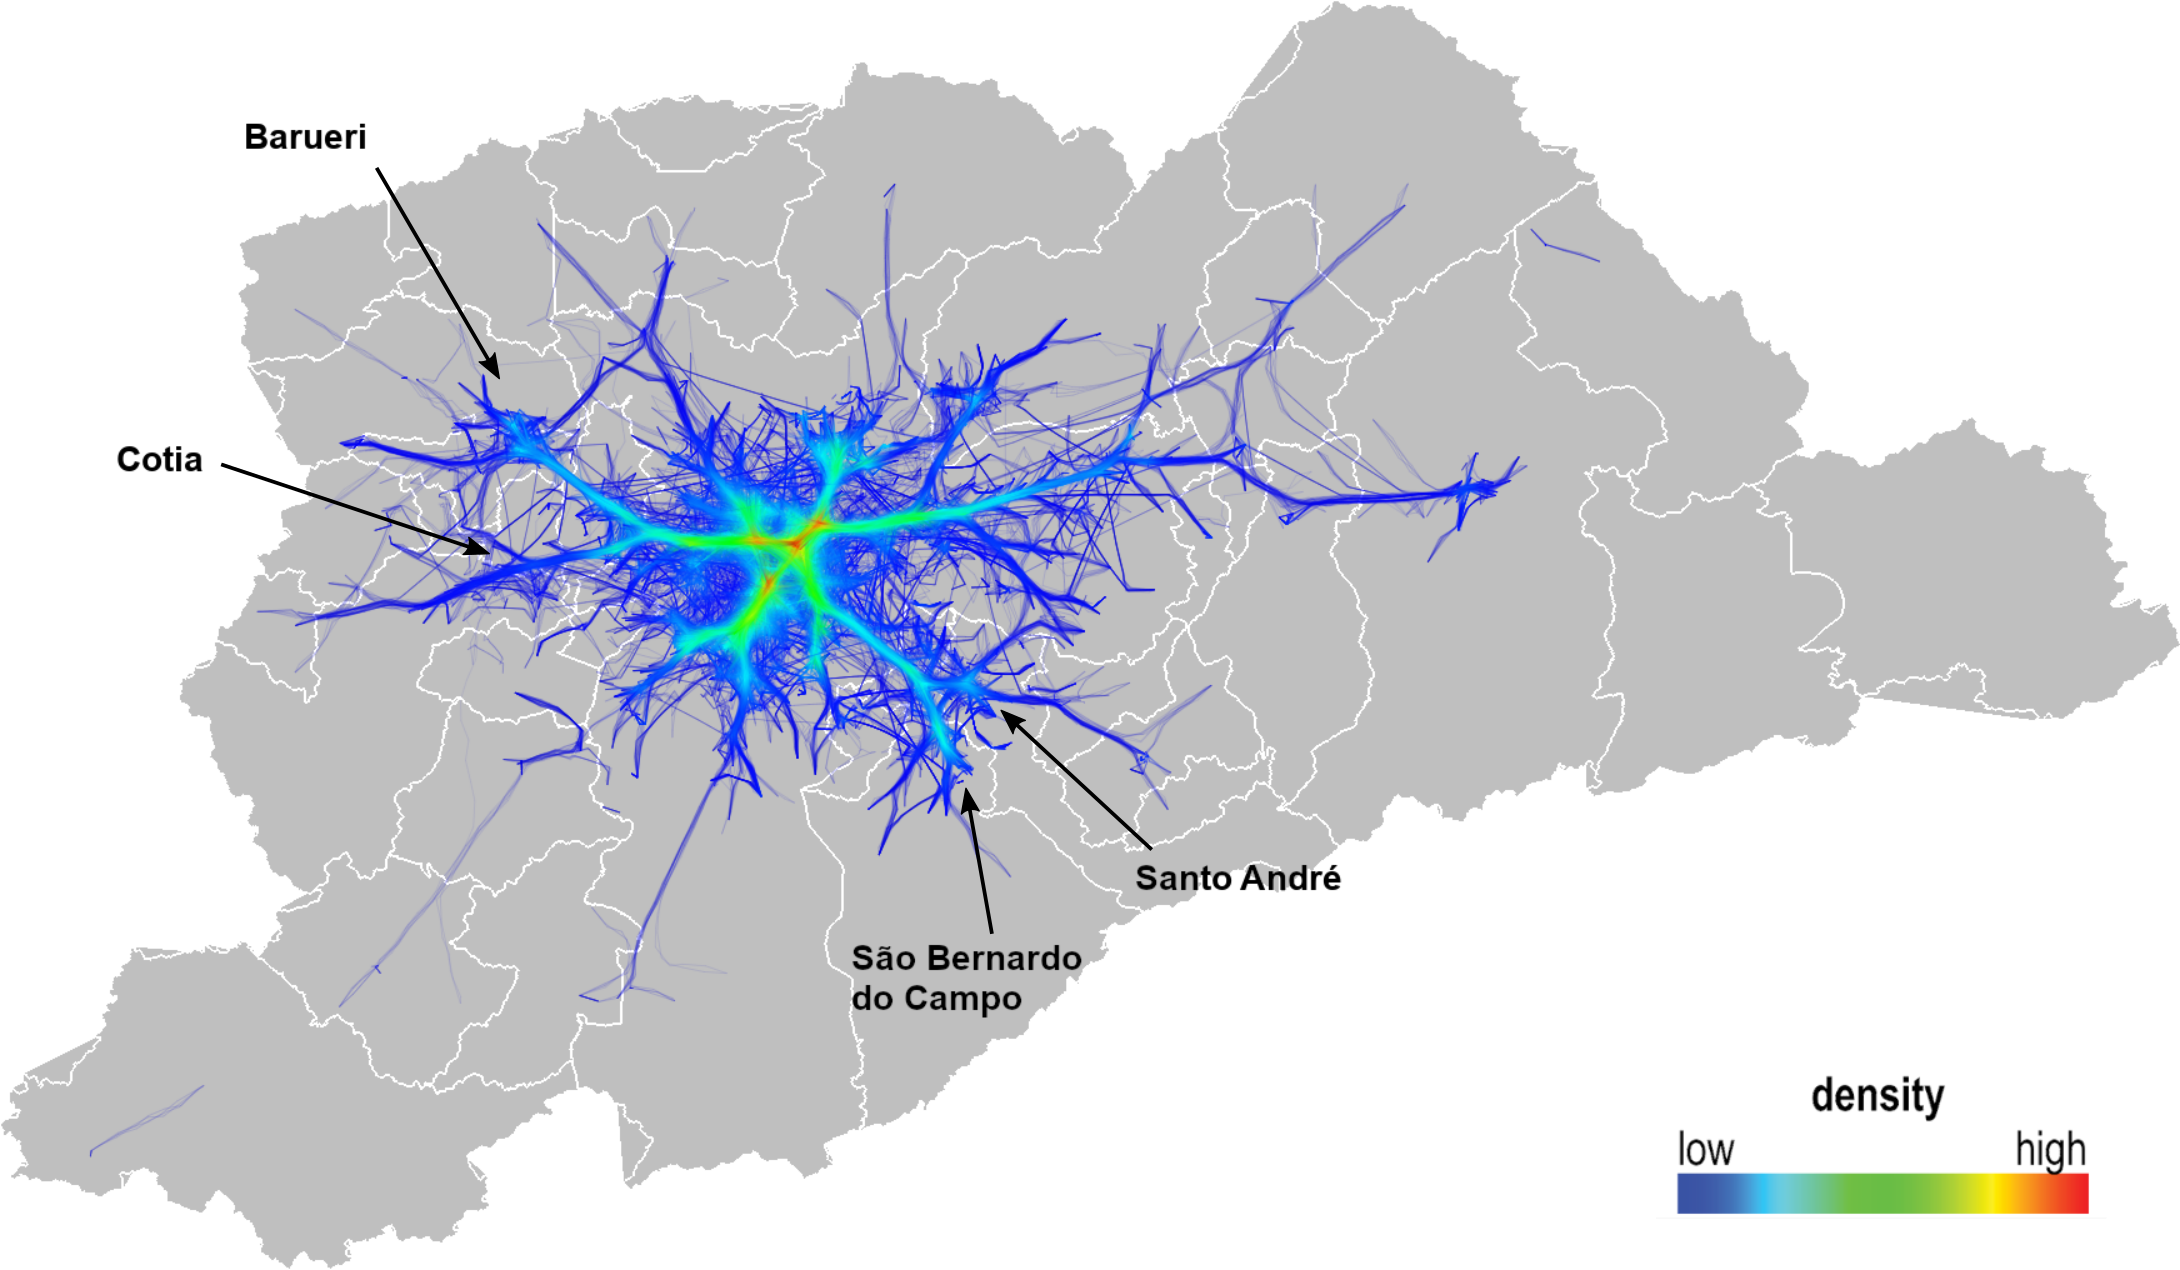
\includegraphics[width=0.98\textwidth]{../figuras/1-class-a.png}
  \caption{Densidade das viagens da classe $A$. \label{fig:becc-a}}
\end{figure}

\begin{figure}[!htb]
  \centering
  \captionsetup{justification=centering}
  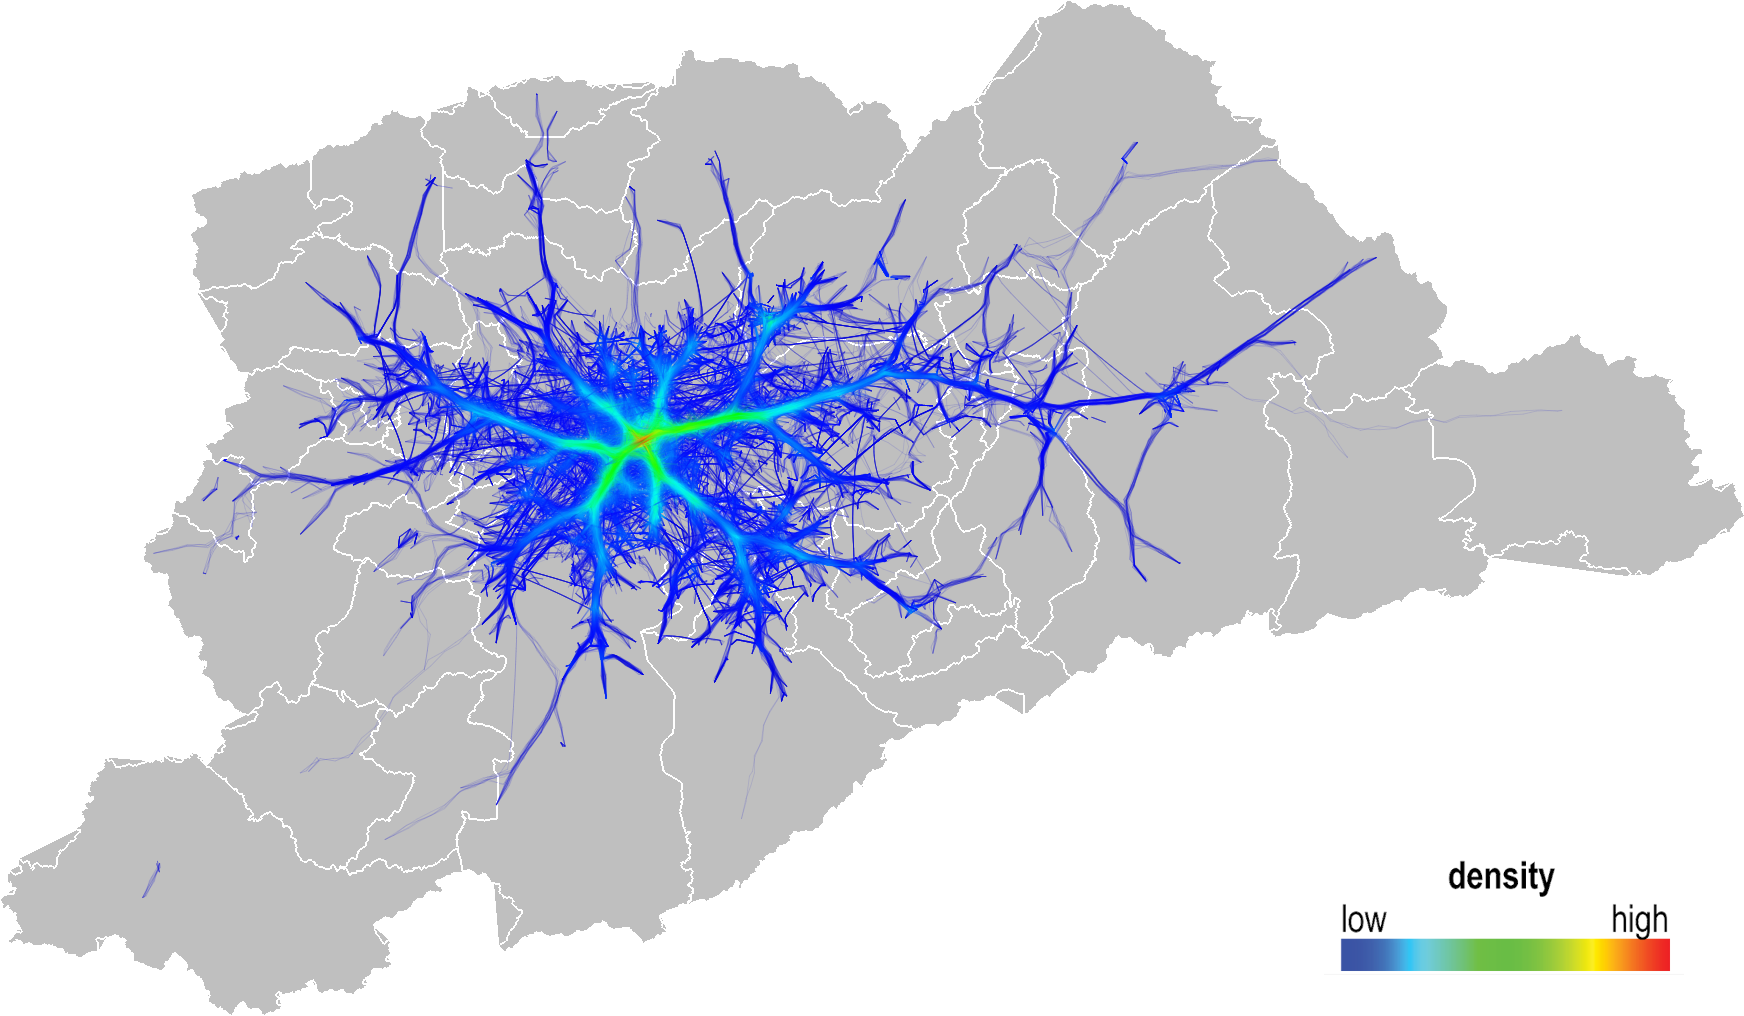
\includegraphics[width=0.98\textwidth]{../figuras/2-class-b1.png}
  \caption{Densidade das viagens da classe $B1$. \label{fig:becc-b1}}
\end{figure}

\begin{figure}[!htb]
  \centering
  \captionsetup{justification=centering}
  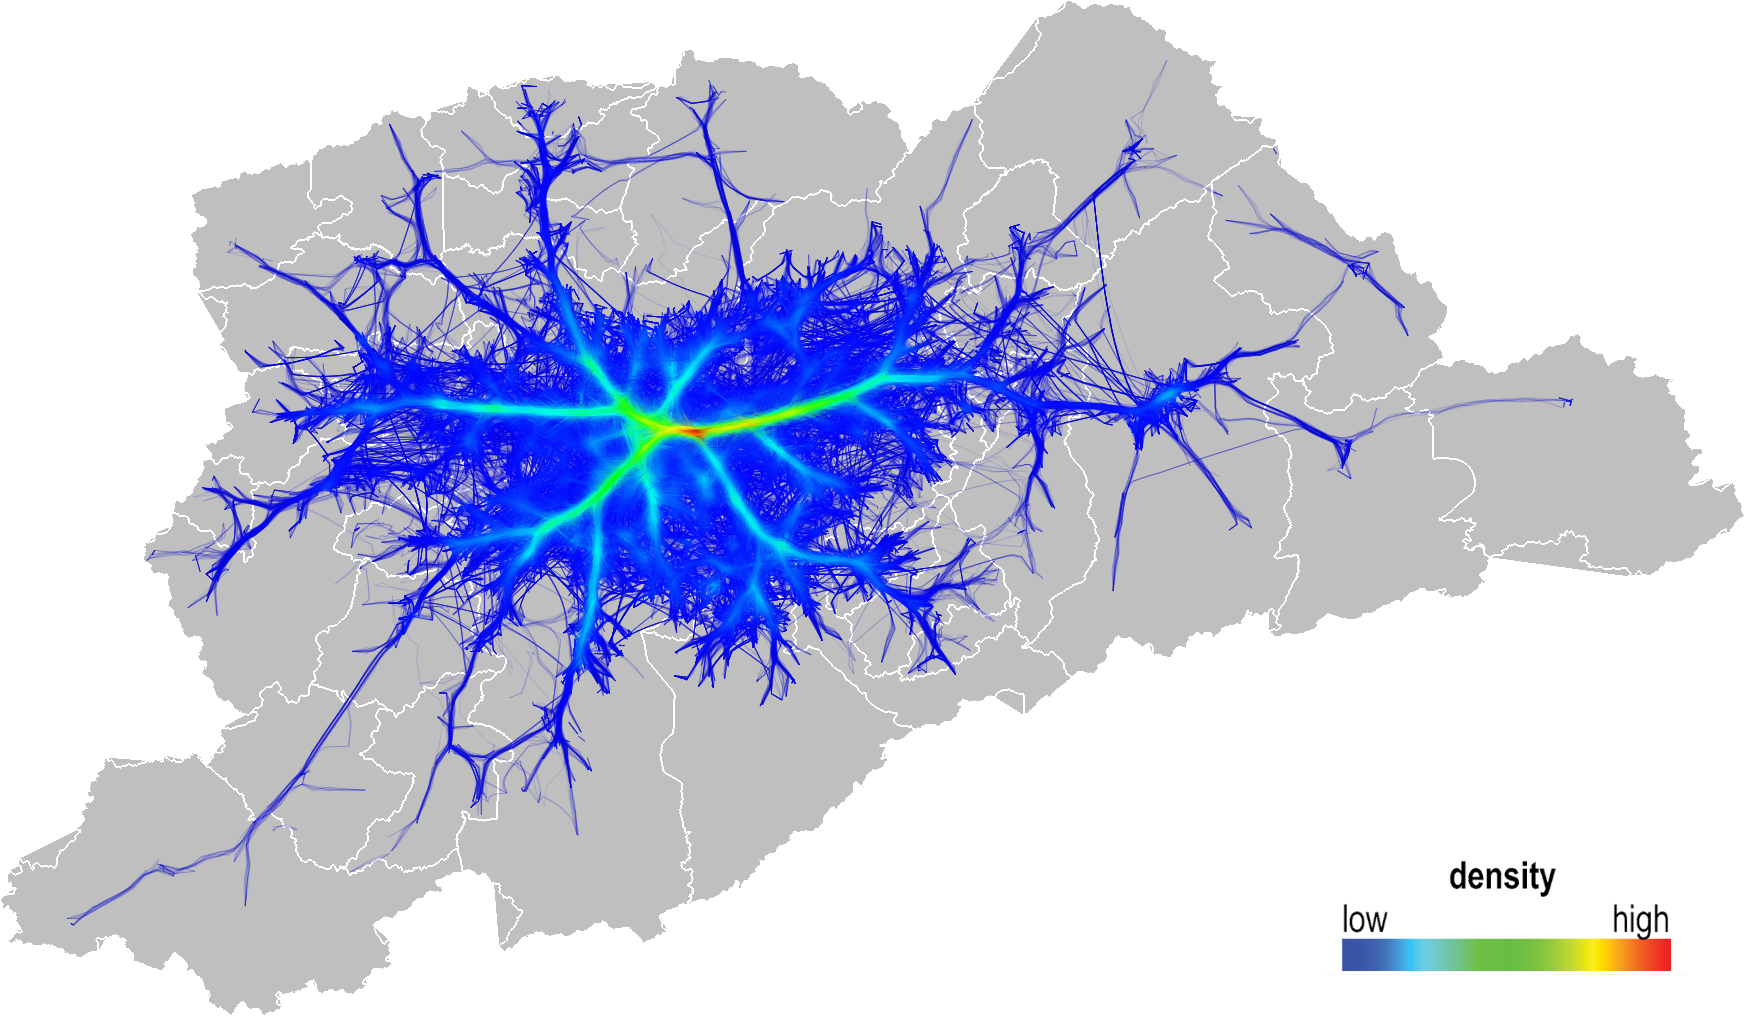
\includegraphics[width=0.98\textwidth]{../figuras/3-class-b2.png}
  \caption{Densidade das viagens da classe $B2$. \label{fig:becc-b2}}
\end{figure}

\begin{figure}[!htb]
  \centering
  \captionsetup{justification=centering}
  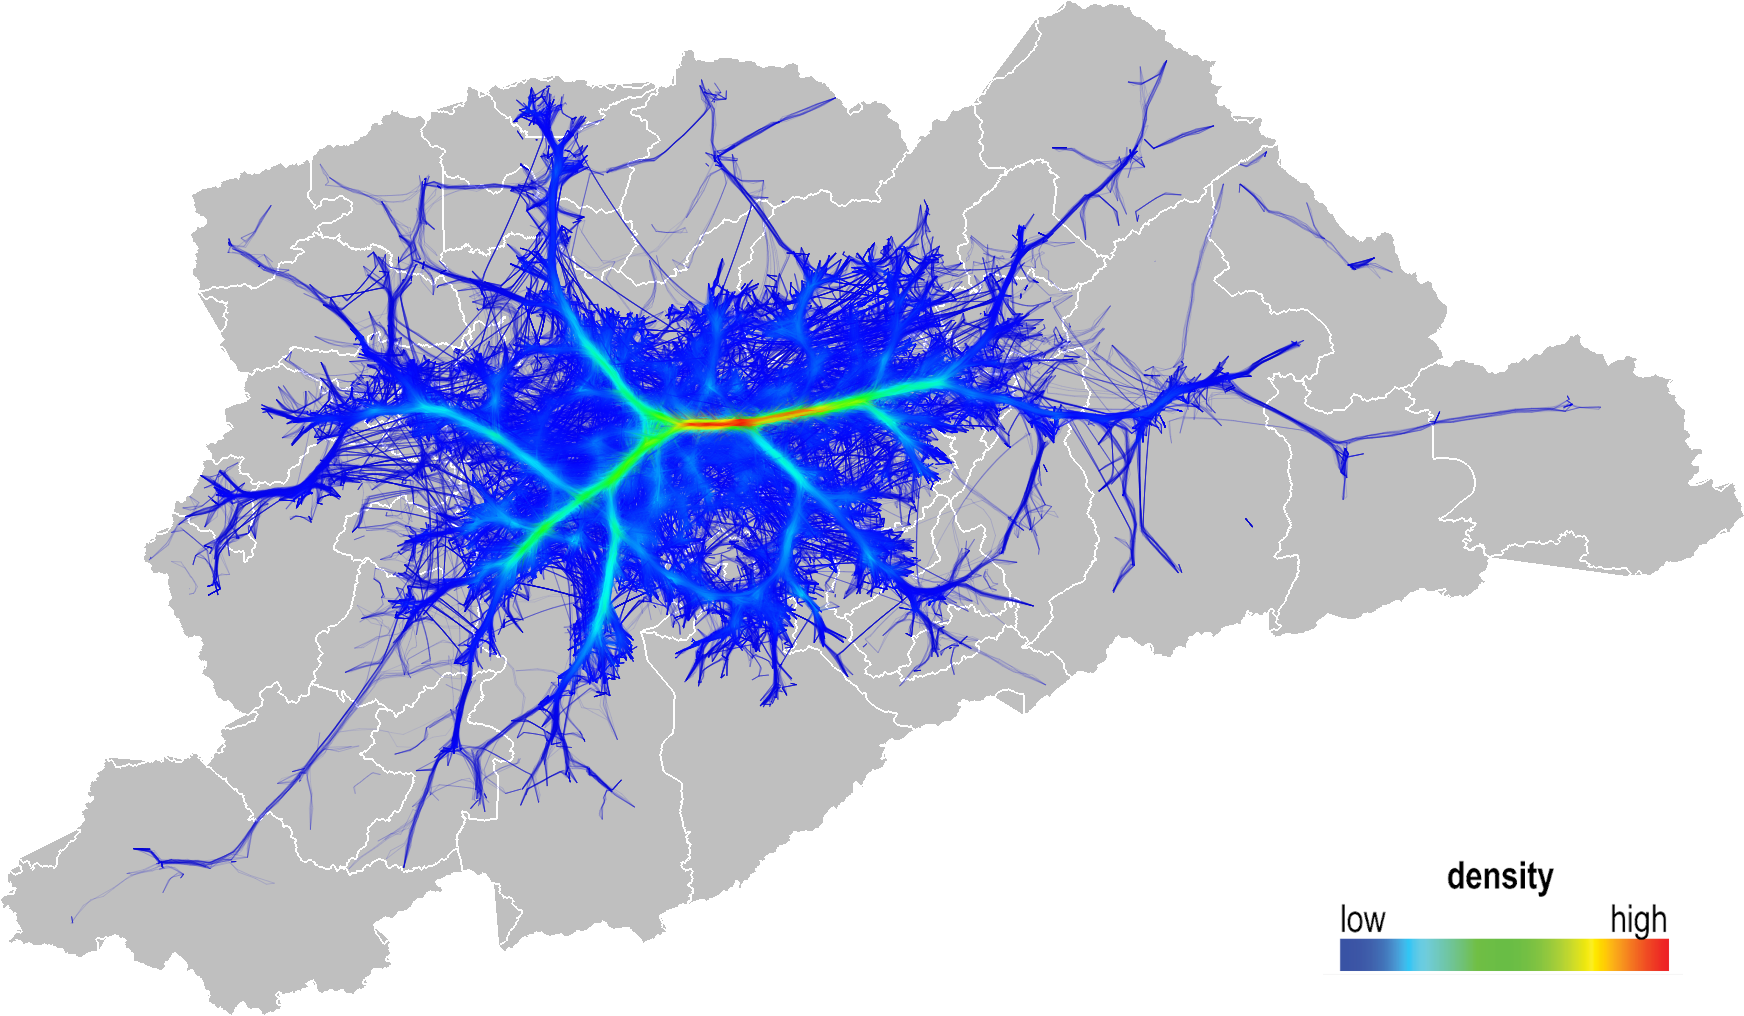
\includegraphics[width=0.98\textwidth]{../figuras/4-class-c1.png}
  \caption{Densidade das viagens da classe $C1$. \label{fig:becc-c1}}
\end{figure}

\begin{figure}[!htb]
  \centering
  \captionsetup{justification=centering}
  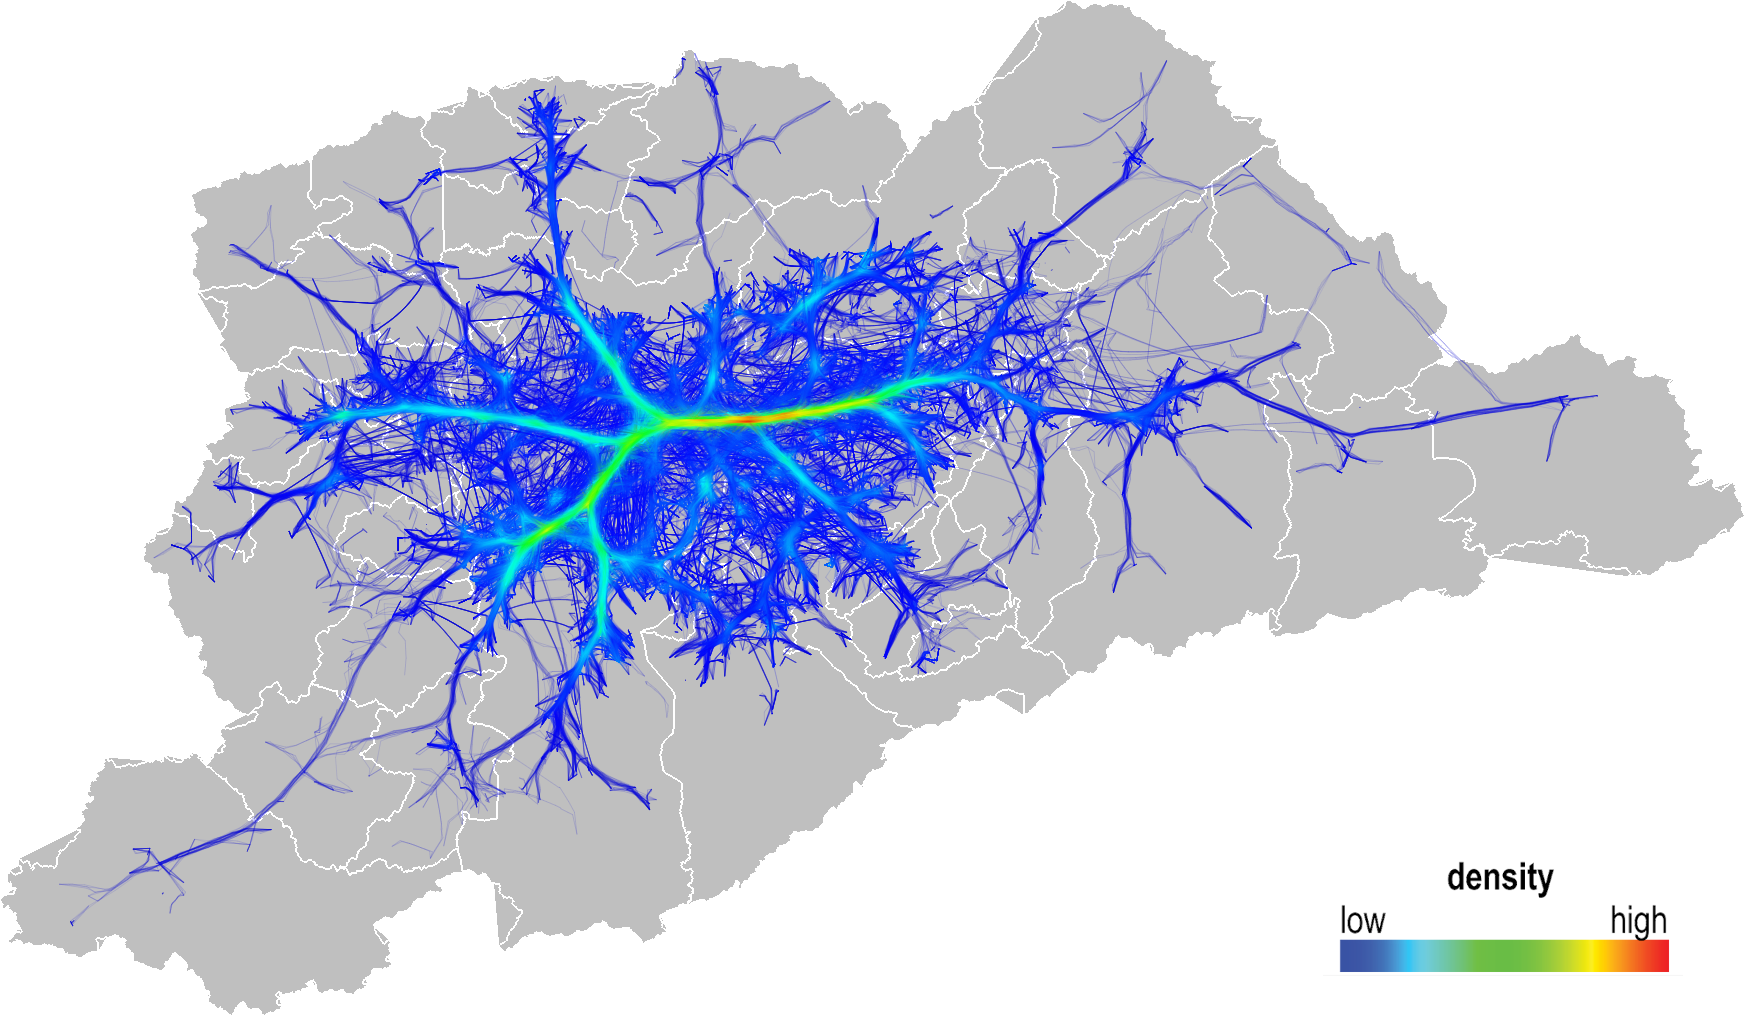
\includegraphics[width=0.98\textwidth]{../figuras/5-class-c2.png}
  \caption{Densidade das viagens da classe $C2$. \label{fig:becc-c2}}
\end{figure}

\begin{figure}[!htb]
  \centering
  \captionsetup{justification=centering}
  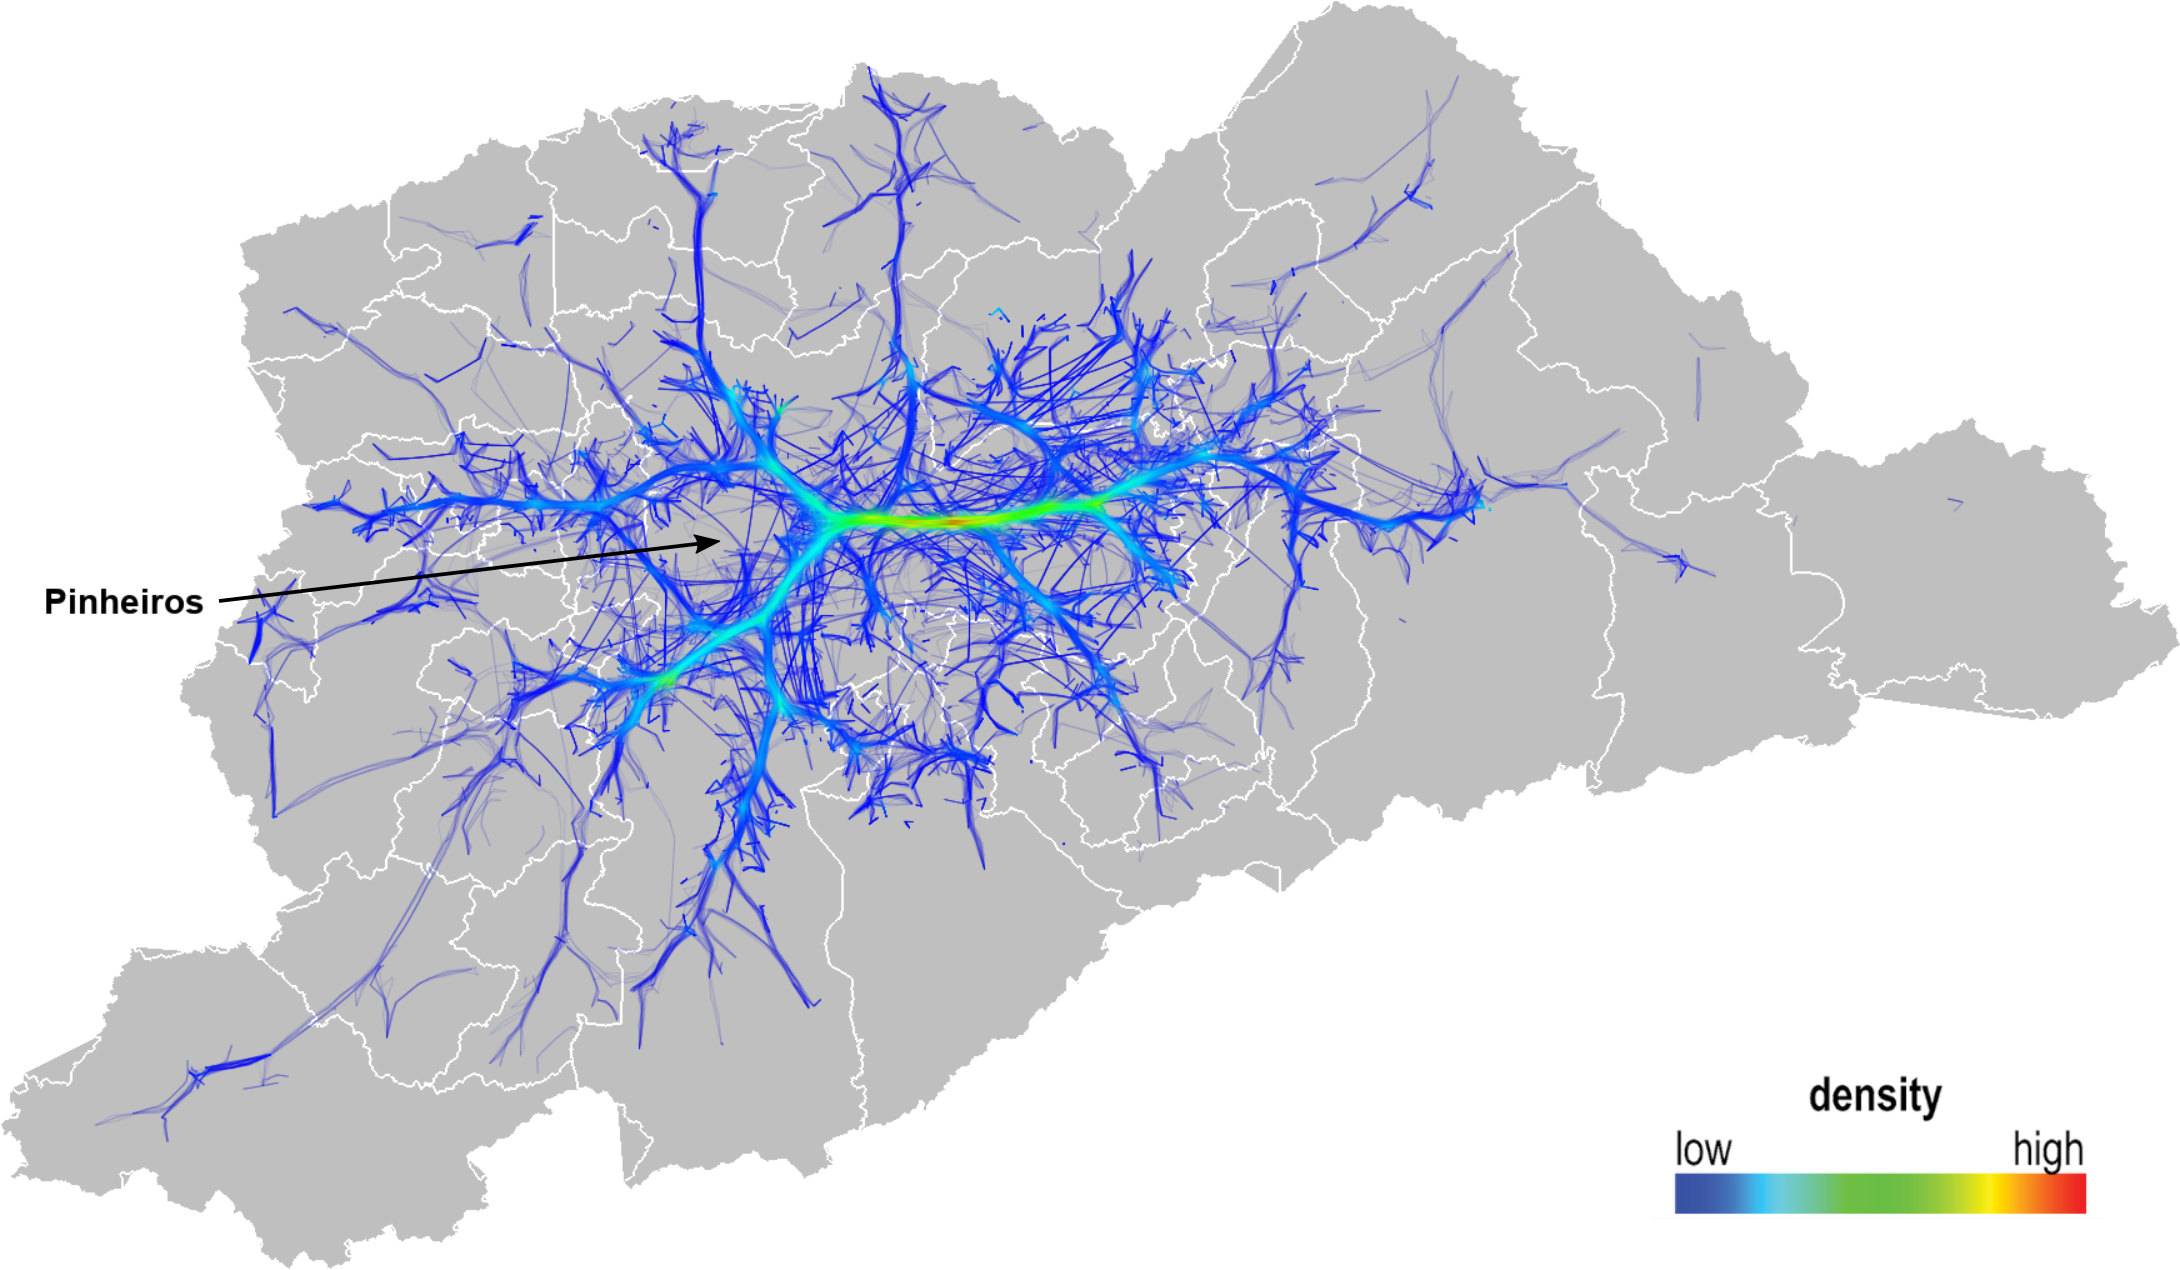
\includegraphics[width=0.98\textwidth]{../figuras/6-class-d-e.png}
  \caption{Densidade das viagens da classe $D$-$E$. \label{fig:becc-d-e}}
\end{figure}

Quando comparamos todos os mapas do nível $A$ ao $D-E$
(Figuras~\ref{fig:becc-a}~to~\ref{fig:becc-d-e}), vemos que os fluxos mais
densos (em vermelho) tendem a se deslocar do centro da capital para a região
leste da cidade. A concentração de fluxos de alta densidade está se espalhando
cada vez mais do centro para as regiões periféricas da RMSP. Mesmo os fluxos
menos densos também se espalhando pela RMSP. No entanto, o mapa $D-E$ mostra que
esses fluxos diminuem consideravelmente (podemos ver pelas linhas menos densas)
para esses estratos sociais. Isso pode indicar que os cidadãos de baixa renda
têm menos acesso ao sistema de mobilidade urbana. Com isso, essas pessoas teriam
menos acesso aos serviços sociais, educacionais, de saúde e culturais da RMSP,
uma vez que esses recursos estão concentrados nas regiões centrais das cidades.
É importante notar que essas regiões centrais também têm mais oportunidades de
emprego. Olhando o mapa $D-E$, podemos ver um notável espaço vazio no centro
oeste da capital. Essa região (distrito de Pinheiros) concentra um grande número
de empregos relacionados à tecnologia da informação e serviços financeiros, o
que requer trabalhadores com níveis de escolaridade alto e médio. Assim, o mapa
mostra que os cidadãos de baixa renda não estão indo para aquela região, o que
reflete a desigualdade de oportunidades que esses cidadãos enfrentam.

\section{Mobilidade de jovens estudantes de diferentes classes sociais}
\label{sec:students}

Um outro uso do \emph{bundling} que fizemos em nosso estudo de visualização de padrões de
mobilidade foi para comparar as viagens de estudantes de diferentes classes
sociais. Para isso, filtramos viagens de indivíduos com idades entre 6 e 18 anos
cujo motivo do deslocamento é o estudo. Então, nós os dividimos em dois grupos,
de alta a moderada renda, que inclui os níveis CCEB $A$, $B1$, $B2$ e $C1$; e os
de baixa renda, que incluem os níveis $C2$ e $D$ - $E$. As
figuras~\ref{fig:students-high}~e~\ref{fig:students-low} mostram os mapas de
densidade para ambos os grupos.

\begin{figure}[!htb]
  \centering
  \captionsetup{justification=centering}
  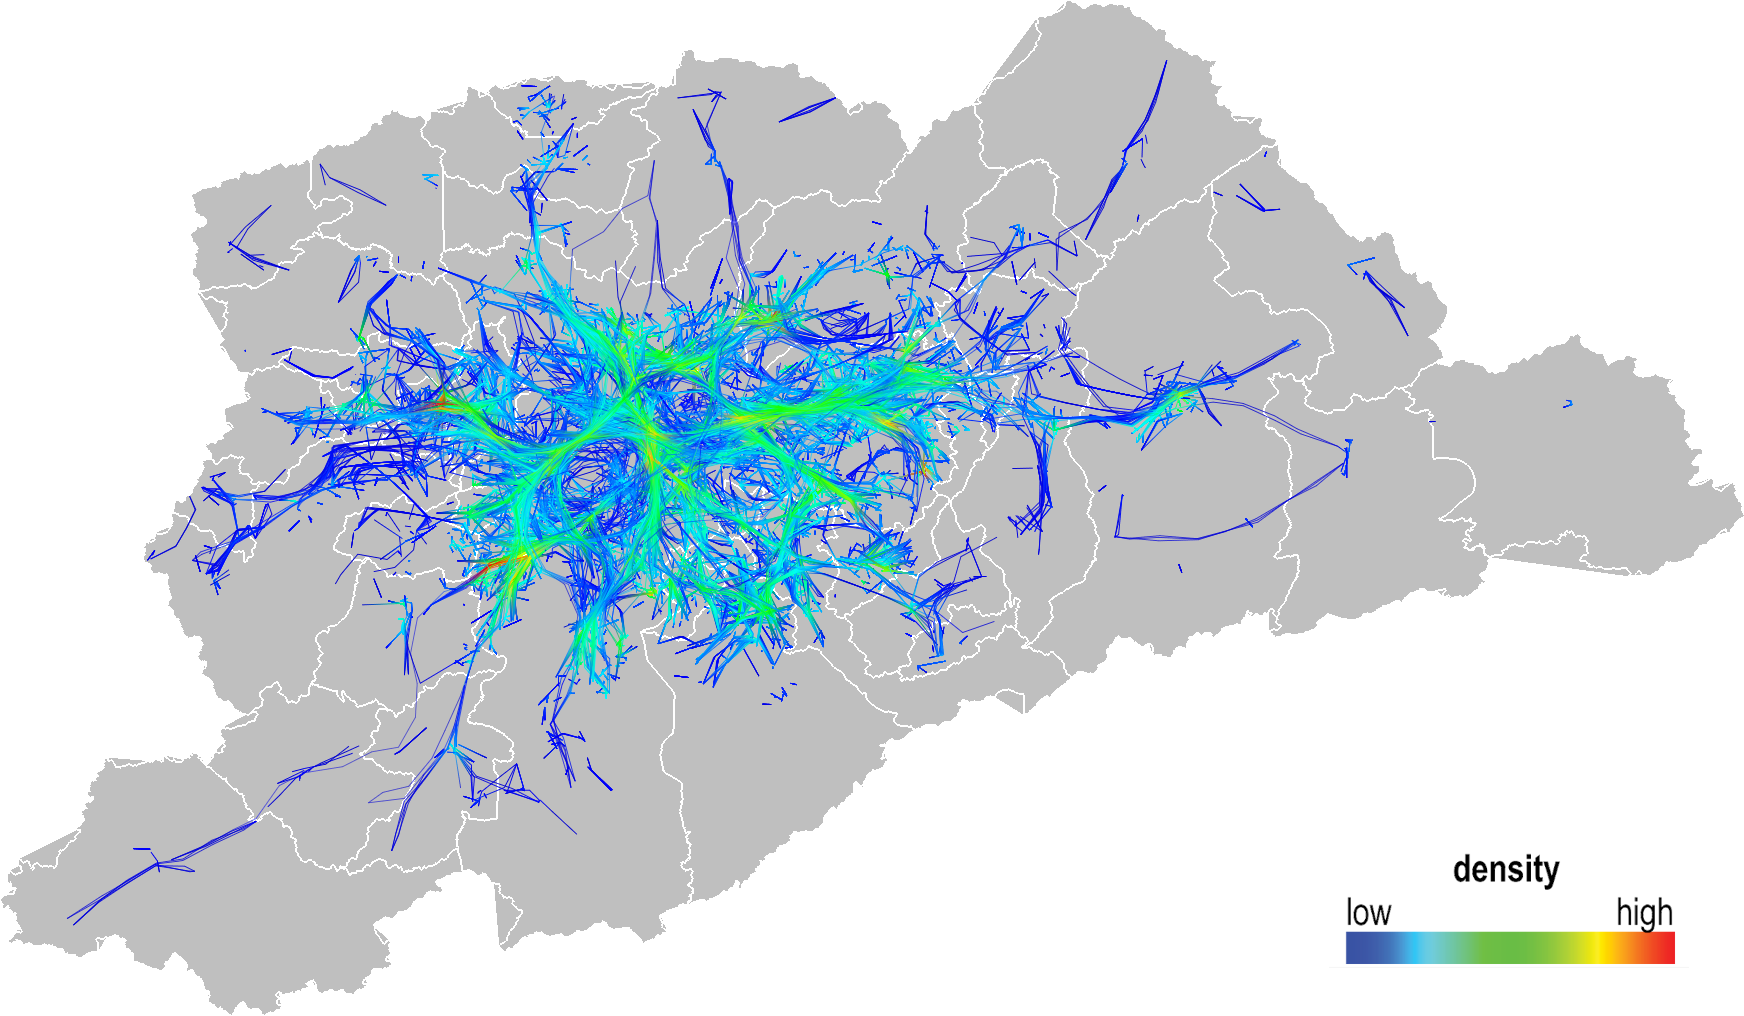
\includegraphics[width=0.98\textwidth]{../figuras/high-income-density-leg.png}
  \caption{Densidade das viagens de estudantes de alta renda. \label{fig:students-high}}
\end{figure}
\vspace*{\floatsep}
\begin{figure}[!htb]
  \centering
  \captionsetup{justification=centering}
  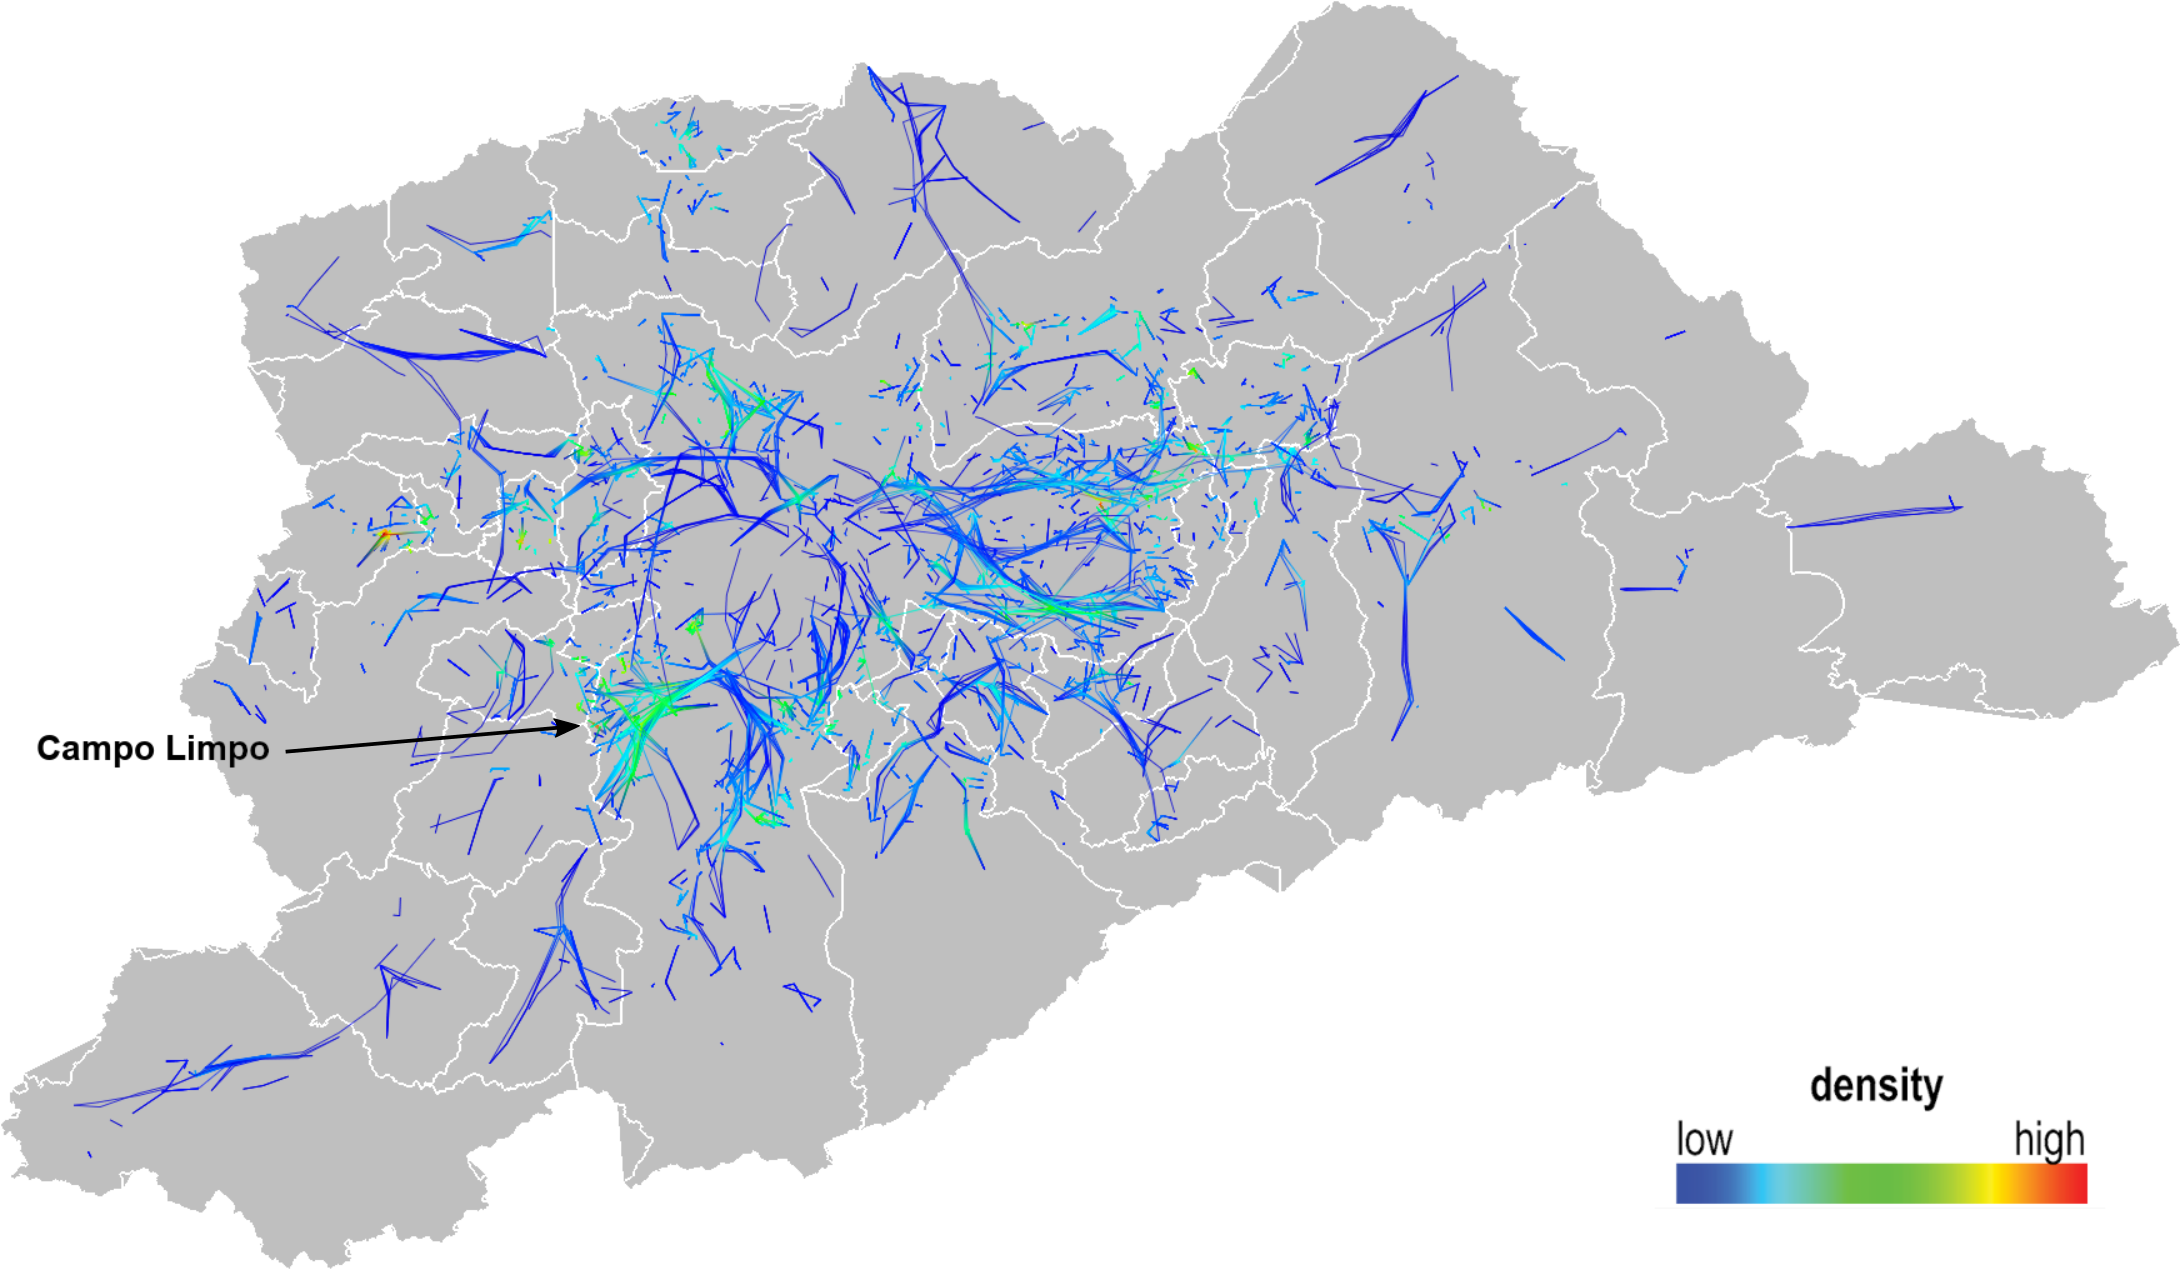
\includegraphics[width=0.98\textwidth]{../figuras/low-income-density-leg.png}
  \caption{Densidade das viagens de estudantes de baixa renda. \label{fig:students-low}}
\end{figure}

Podemos ver no mapa da Figura~\ref{fig:students-high} que a densidade dos fluxos
do grupo de alunos de alta a moderada renda se mostram muito mais densos e
espalhados pela a região central da RMSP. Esta parte da RMSP concentra a maioria
das escolas particulares, universidades e faculdades. Já o mapa de densidade de
alunos de baixa renda (Figura~\ref{fig:students-low}) mostra uma mobilidade bem
mais limitada em comparação com os alunos de alta renda, com alguns fluxos
interligados ao centro da capital, mas a maioria dos fluxos densos dessa classe
estão mais presentes nas periferias da capital e também nas cidades vizinhas.
Apesar das diferenças, podemos ver que há concentração dos dois grupos na região
sudoeste, onde ficam os bairros do distrito de Campo Limpo.

Podemos observar que há muito mais trilhas para os alunos de alta renda
(Figura~\ref{fig: students-high}) do que para alunos de baixa renda
(Figura~\ref{fig:students-low}). Os estudantes de renda alta também viajam
grandes distâncias para estudar, o que indica que podem escolher com mais
flexibilidade onde estudar. Este fato é corroborado por estudos de mobilidade
urbana que indicam que pessoas com melhores condições financeiras têm mais
mobilidade do que aquelas com condições mais precárias \cite{carruthers2005,
lucas2016}.

Vale ressaltar que as escolas públicas da RMSP estão distribuídas pela região
central e periférica das cidades. Em geral, o sistema público busca alocar as
matrículas dos alunos nessas escolas de acordo com a proximidade de suas
residências. Assim, eles não precisam viajar longas distâncias para chegar às
suas escolas. Além disso, as escolas públicas apresentam desempenho educacional
inferior ao das escolas particulares de São Paulo. Assim, cidadãos com melhores
condições financeiras costumam colocar seus filhos em escolas particulares.

A escassez de fluxos de alunos de baixa renda ascende questionamentos. Ela pode
ser uma indicação de que esta classe da população não têm oportunidades iguais
de estudo. Também não costumam ir para a região central da cidade e, portanto,
têm menos acesso a universidades e faculdades complementares. Essa desigualdade
de oportunidades provavelmente afetará os empregos e as condições econômicas
desses alunos.

\section{Direção das viagens nos horários de pico}
\label{sec:peak-hours}

Conforme mostramos anteriormente na Figura~\ref{fig:trips_by_hour} da
Seção~\ref{sec:pesquisa-od}, distribuição das viagens por hora do dia tem dois picos
principais, entre 6 e 9h e entre 17 e 20h. No entanto, essa tabela agregada não
fornece informações sobre como os padrões de mobilidade nos horários de pico
podem ser diferentes. Para visualizar esses dados, criamos dois conjuntos de
dados, um pra cada intervalo, e aplicamos \emph{bundling} em cada conjunto
separadamente. Codificamos a direção a das viagens em cores, similar ao
apresentado na Figura~\ref{fig:attributes-direction}, da
Seção~\ref{sec:length-direction}.

\begin{figure}[!htb]
  \centering
  \captionsetup{justification=centering}
  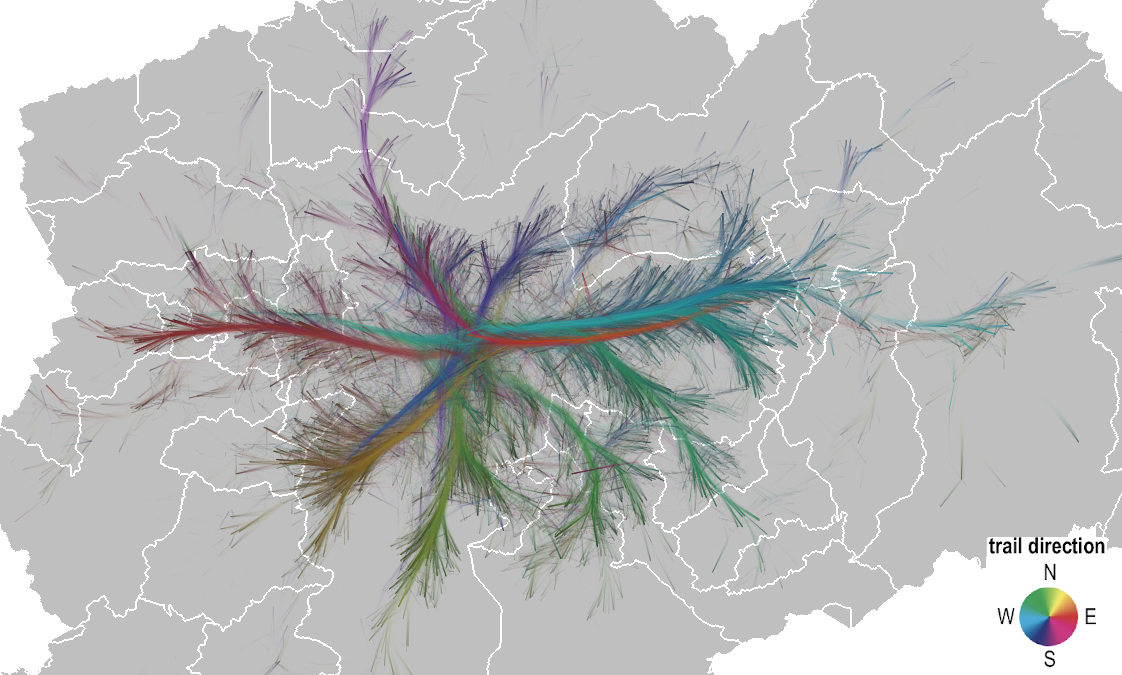
\includegraphics[width=0.98\textwidth]{../figuras/peak-hours-6h-to-9h-direction-leg.png}
  \caption{Direção das viagens entre 6 e 9 da manhã. \label{fig:peak-hours-6h-9h}}
\end{figure}
\vspace*{\floatsep}
\begin{figure}[!htb]
  \centering
  \captionsetup{justification=centering}
  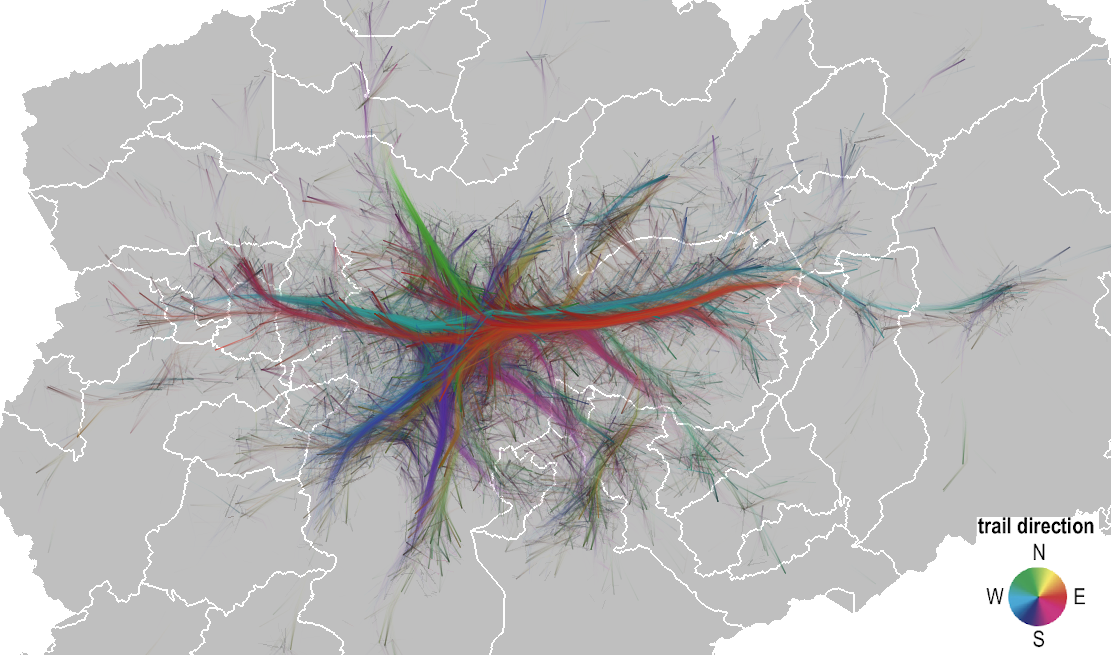
\includegraphics[width=0.98\textwidth]{../figuras/peak-hours-17h-to-20h-direction-leg.png}
  \caption{Direção das viagens entre 17 e 20h. \label{fig:peak-hours-17h-20h}}
\end{figure}

Comparando as horas de pico, podemos ver que os fluxos matinais indo para o
centro da RMSP (Figura~\ref{fig:peak-hours-6h-9h}, fluxo ciano vindo do leste)
são geralmente mais densos e mais longos do que os fluxos vindos do Centro RMSP
durante o pico da tarde/noite (Figura~\ref{fig:peak-hours-17h-20h}, fluxo
vermelho). Isso sugere que na da manhã as pessoas têm pressa para chegar ao
trabalho, ao passo que têm menos pressa para voltar para casa (ou para outros
destinos como escolas ou academia) no período da tarde/noite.

\section{Densidade das viagens por modo de transporte}
\label{sec:mode}

Um outro interessante atributo presente nos dados da pesquisa OD17 é o modo de
transporte. Comparamos então padrões de fluxo para quatro modos de transporte
diferentes: pedestres, bicicletas, carros e metrô. Nas
figuras~\ref{fig:mode-pedestrian}~até~\ref{fig:mode-subway} utilizamos o
\emph{bundling} para visualizar a densidade dos fluxos de cada um dos tipos de
transporte. Diferentemente do que apresentamos na seção~\ref{sec:coloring}, onde
aplicamos \emph{bundling} em todo o conjunto de dados e utilizamos filtros para
selecionar categorias de transporte de interesse, aqui utilizamos a estratégia de
particionamento para visualizar cada conjunto separadamente. Com isso damos
ênfase às características de cada subconjunto em específico, já que o
mapa de densidade é calculado com os valores daquela única classe de atributos.
 
\begin{figure}[!htb]
  \centering
  \captionsetup{justification=centering}
  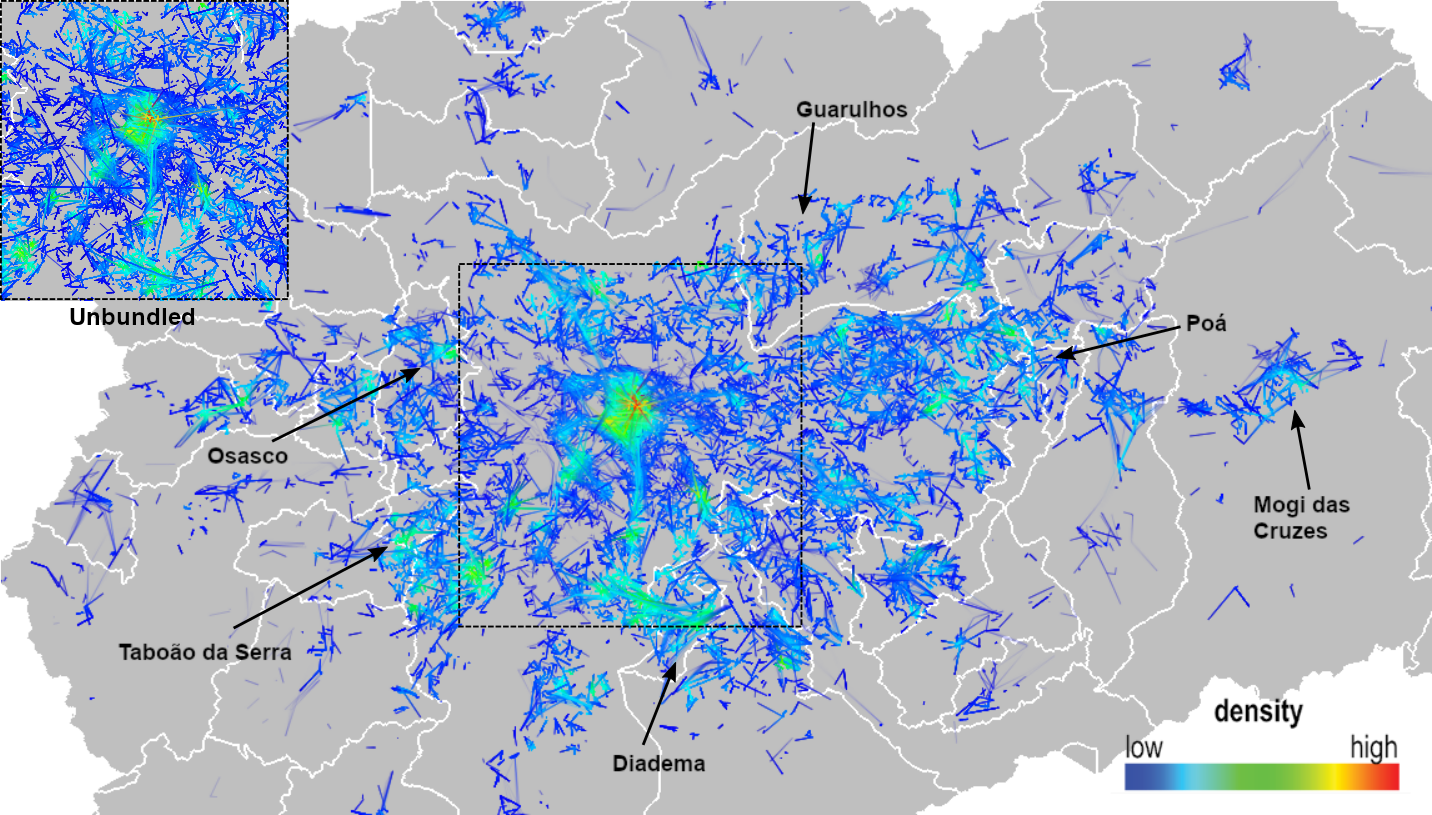
\includegraphics[width=0.98\textwidth]{../figuras/mode-pedestrian-density-leg.png}
  \caption{Densidade das viagens de pedestres. \label{fig:mode-pedestrian}}
\end{figure}

\begin{figure}[!htb]
  \centering
  \captionsetup{justification=centering}
  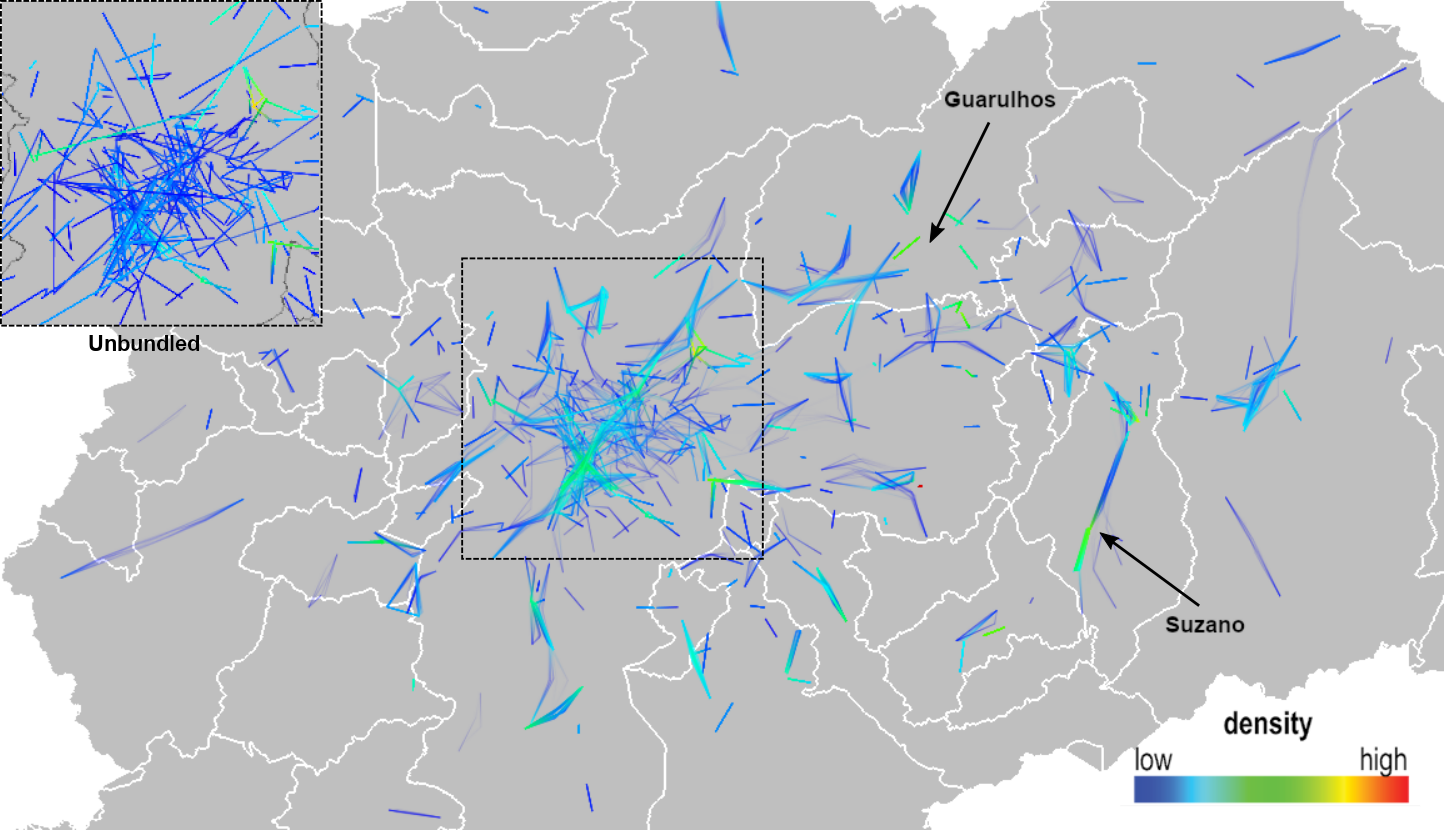
\includegraphics[width=0.98\textwidth]{../figuras/mode-bike-density-leg.png}
  \caption{Densidade das viagens de bicicleta \label{fig:mode-bike}}
\end{figure}

\begin{figure}[!htb]
  \centering
  \captionsetup{justification=centering}
  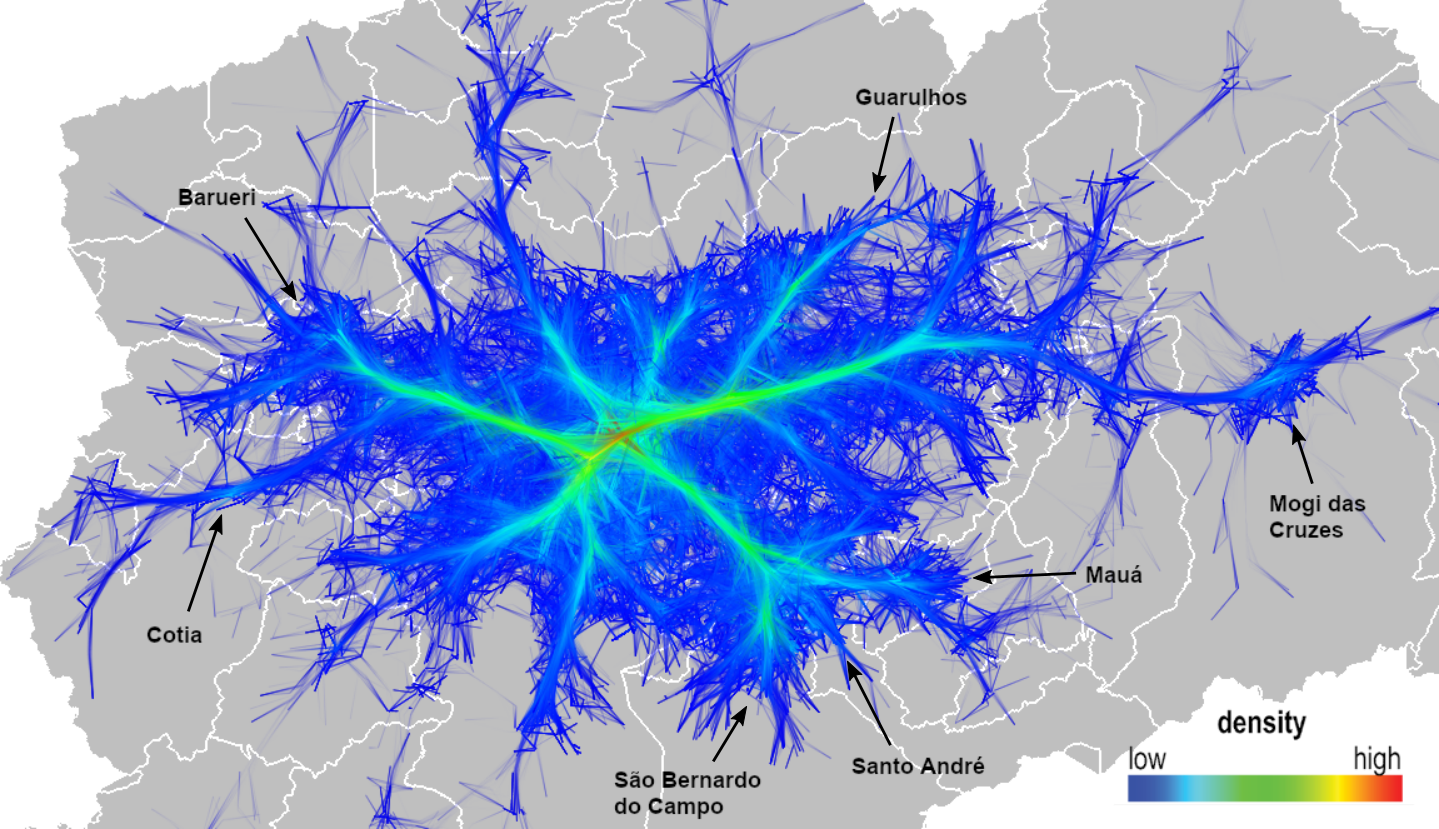
\includegraphics[width=0.98\textwidth]{../figuras/mode-car-density-leg.png}
  \caption{Densidade das viagens de carro. \label{fig:mode-car}}
\end{figure}

\begin{figure}[!htb]
  \centering
  \captionsetup{justification=centering}
  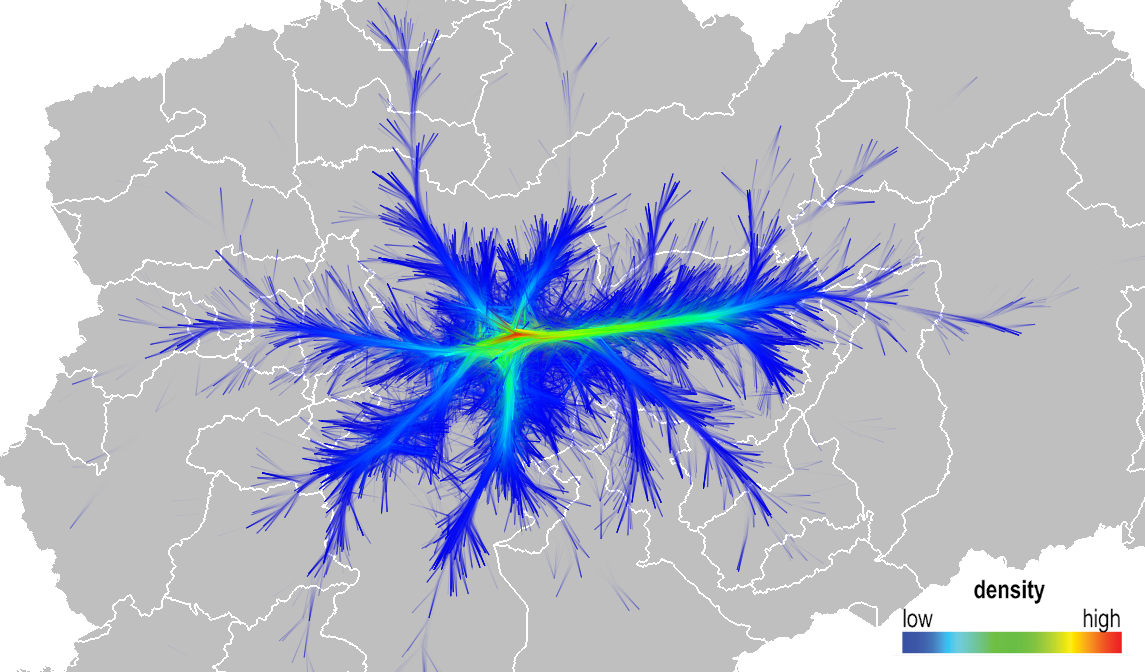
\includegraphics[width=0.98\textwidth]{../figuras/mode-subway-density-leg.png}
  \caption{Densidade das viagens de metrô. \label{fig:mode-subway}}
\end{figure}

As viagens de pedestres (Figura~\ref{fig:mode-pedestrian}) formam várias
``ilhas'' de baixa densidade espalhadas pela RMSP, sendo a mais densa (em vermelho)
no centro da capital. A maioria das trilhas são curtas, o que
é esperado para pedestres. No entanto, vemos alguns \emph{bundles} mais longos se estendendo
entre o centro da capital e as regiões sul e norte da cidade. Alguns fluxos mais densos também
estão presentes nas cidades vizinhas de Diadema, Taboão da Serra, Osasco,
Guarulhos, Poá e Mogi das Cruzes. Examinando mais de perto, observamos que
os fluxos densos combinam geograficamente com áreas centrais das cidades e as áreas comerciais. Essas
informações podem ser úteis para localizar locais que possam merecer a atenção
dos governos locais para proporcionar melhorias aos pedestres.

Como a maioria das viagens de pedestres são curtas, a técnica de \emph{bundling}
forma poucos fluxos sobre a RMSP. Usar o \emph{bundling} para essas viagens
curtas resulta em alguns poucos fluxos de baixa densidade, o que é menos útil em
comparação com viagens longas. Em casos como este, pode não ser necessário usar
o \emph{bundling}. Na área superior esquerda da
Figura~\ref{fig:mode-pedestrian}, temos destacadas as viagens OD da área central da
cidade sem utilização do \emph{bundling}; podemos ver que são quase idênticas
aos resultados com \emph{bundling} aplicado.

Com uma média de menos de três quilômetros, as viagens de bicicleta
(Figura~\ref{fig:mode-bike}) exibem padrões semelhantes aos de pedestres.  Nesta
figura, vemos alguns fluxos estreitos na área central da capital. Existem também
alguns fluxos mais salientes no Nordeste da capital e nas cidades vizinhas de
Suzano e Guarulhos. No entanto, comparando a Figura~\ref{fig:mode-bike} com
todos os outros meios de transporte, vemos imediatamente que as viagens de
bicicleta são de longe as menos numerosas e exibem um padrão muito mais esparso,
com poucos caminhos em forma de estrela onde muitas trajetórias se encontram.
Isso sugere que a infraestrutura de ciclismo é bastante limitada e fragmentada.
No canto superior esquerdo da Figura~\ref{fig:mode-bike} também mostramos
as viagens sem utilização do \emph{bundling}.

As viagens de carro (Figura~\ref{fig:mode-car}) mostram um padrão
semelhante ao que exibe todo o conjunto de dados, (ver Figura~\ref{fig:bundled-graph-density}).
Para começar, isso indica que os carros são a forma
dominante de transporte na RMSP, respondendo pelos principais padrões de
tráfego. Os fluxos de maior densidade ocorrem no centro da capital. Podemos observar diversos
fluxos de alta densidade ligando o Centro às demais regiões da capital, e também
indo e vindo das cidades de Guarulhos, Barueri, Cotia, São Bernardo do Campo,
Santo André, Mauá, e Mogi das Cruzes. Em comparação com todos os outros
modos de transporte, os carros mostram um padrão muito mais ``espalhado'' que
cobre áreas muito grandes, indicando que os carros são o modo de transporte
predominante na maioria das partes da RMSP.

Por fim, as viagens de metrô (Figura~\ref{fig:mode-subway}) apresentam um forte
padrão em forma de estrela, com fluxos de alta densidade que ligam a capital às
cidades vizinhas, devido à integração do sistema metroviário com o trem sistema
(vide Seção~\ref{sec:trail-overlap}). Comparado aos outros quatro modos de
transporte, o metrô apresenta uma estrutura de padrão de viagem mais clara e
simples.

\section{Visualização por motivo da viagem}
\label{sec:dist_reasons}
Um outro atributo da pesquisa OD 17 que também achamos interessante em nossa
análise foi o motivo das viagens feitas. Observar a mobilidade urbana sobre essa
informação o pode revelar padrões comportamentais interessantes da população. A
seguir, estudamos as distâncias das viagens feitas por diferentes motivos, e que
tipos de padrões elas exibem. Para isso, criamos visualizações a partir dos
dados OD17 particionados por trabalho, saúde, educação e compras. As
figuras~\ref{fig:reason-work}~a~\ref{fig:reason-shopping} mostram os resultados.

As viagens de trabalho (Figura~\ref{fig:reason-work}) são geralmente mais longas
do que as outras razões de viagens e também cobrem uma área maior (veja a
aglomeração central na figura). Curiosamente, as viagens mais longas, entre o
lado leste e o centro da cidade (feixe vermelho), são um padrão semelhante às
viagens mais longas para saúde e educação. As viagens por motivos de saúde
(Figura~\ref{fig:reason-health}) são mais esparsas do que as relacionadas com o
trabalho e também apresentam um padrão mais estrelado, com longos fluxos
conectando-se à área central. Argumentamos que isso pode indicar que as regiões
periféricas não são bem servidas por serviços de saúde. As viagens por motivos
de estudo (Figura~\ref{fig:reason-education}) apresentam as maiores distâncias
entre as regiões Nordeste e Oeste da RMSP. Seu padrão apresenta ser algo
intermediário entre as viagens de trabalho e saúde. Curiosamente, as viagens
educacionais mostram várias ``voltas'' no centro da RMSP. Finalmente, as viagens
de compras (Figura~\ref{fig:reason-shopping}) mostram os padrões menos densos e,
em geral, também os mais curtos, mas com algumas exceções como o feixe vermelho
(importante) conectando o centro ao nordeste. Isso indica que, ao contrário da
saúde, educação e trabalho, os estabelecimentos comerciais (que na verdade são
da iniciativa privada) estão mais bem distribuídos na RMSP. Isso mostra que as
visualizações agregadas - como as feitas com \emph{bundling} - são úteis não
apenas quando mostram a \emph{presença} de certos dados, \emph{por exemplo}
viagens ligando regiões distantes; a \emph{ausência} de padrões também é
igualmente interessante, como no caso da falta de longas viagens por motivo de
compras.

\begin{figure}[!htb]
\centering
\captionsetup{justification=centering}
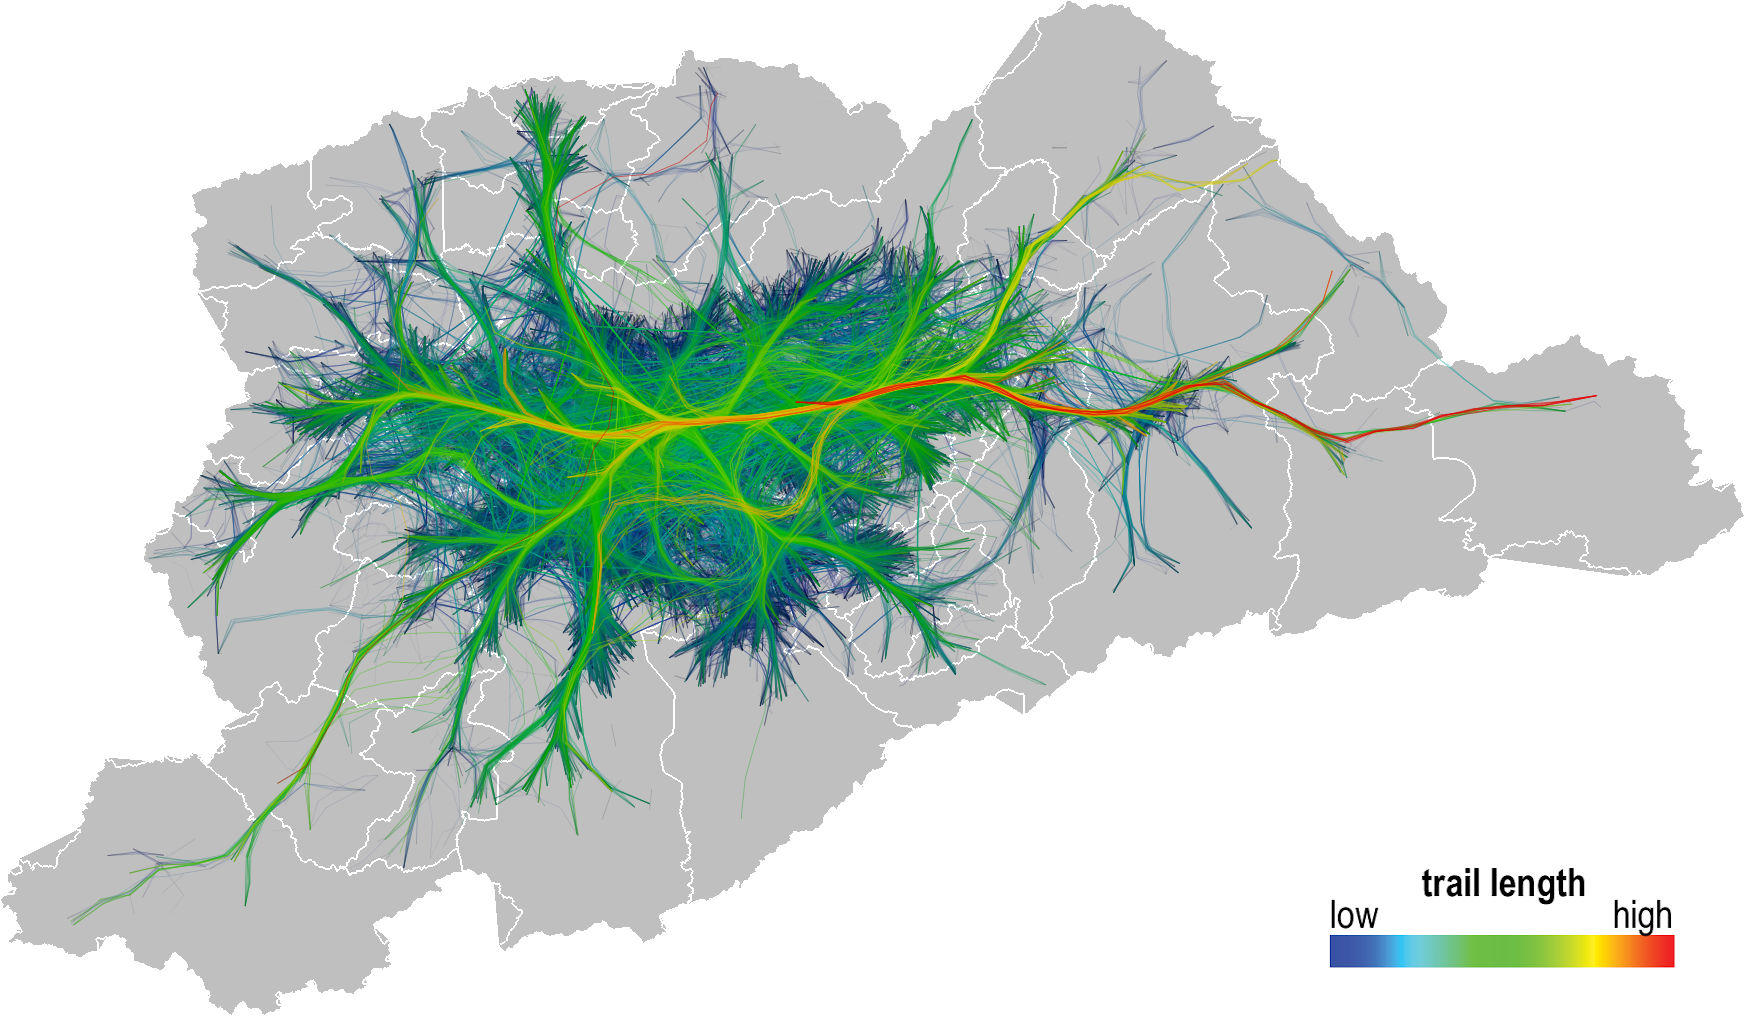
\includegraphics[width=0.98\textwidth]{../figuras/reason-work-leg.png}
\caption{Distâncias das viagens por motivo de trabalho.\label{fig:reason-work}}
\end{figure}
  
\begin{figure}[!htb]
\centering
\captionsetup{justification=centering}
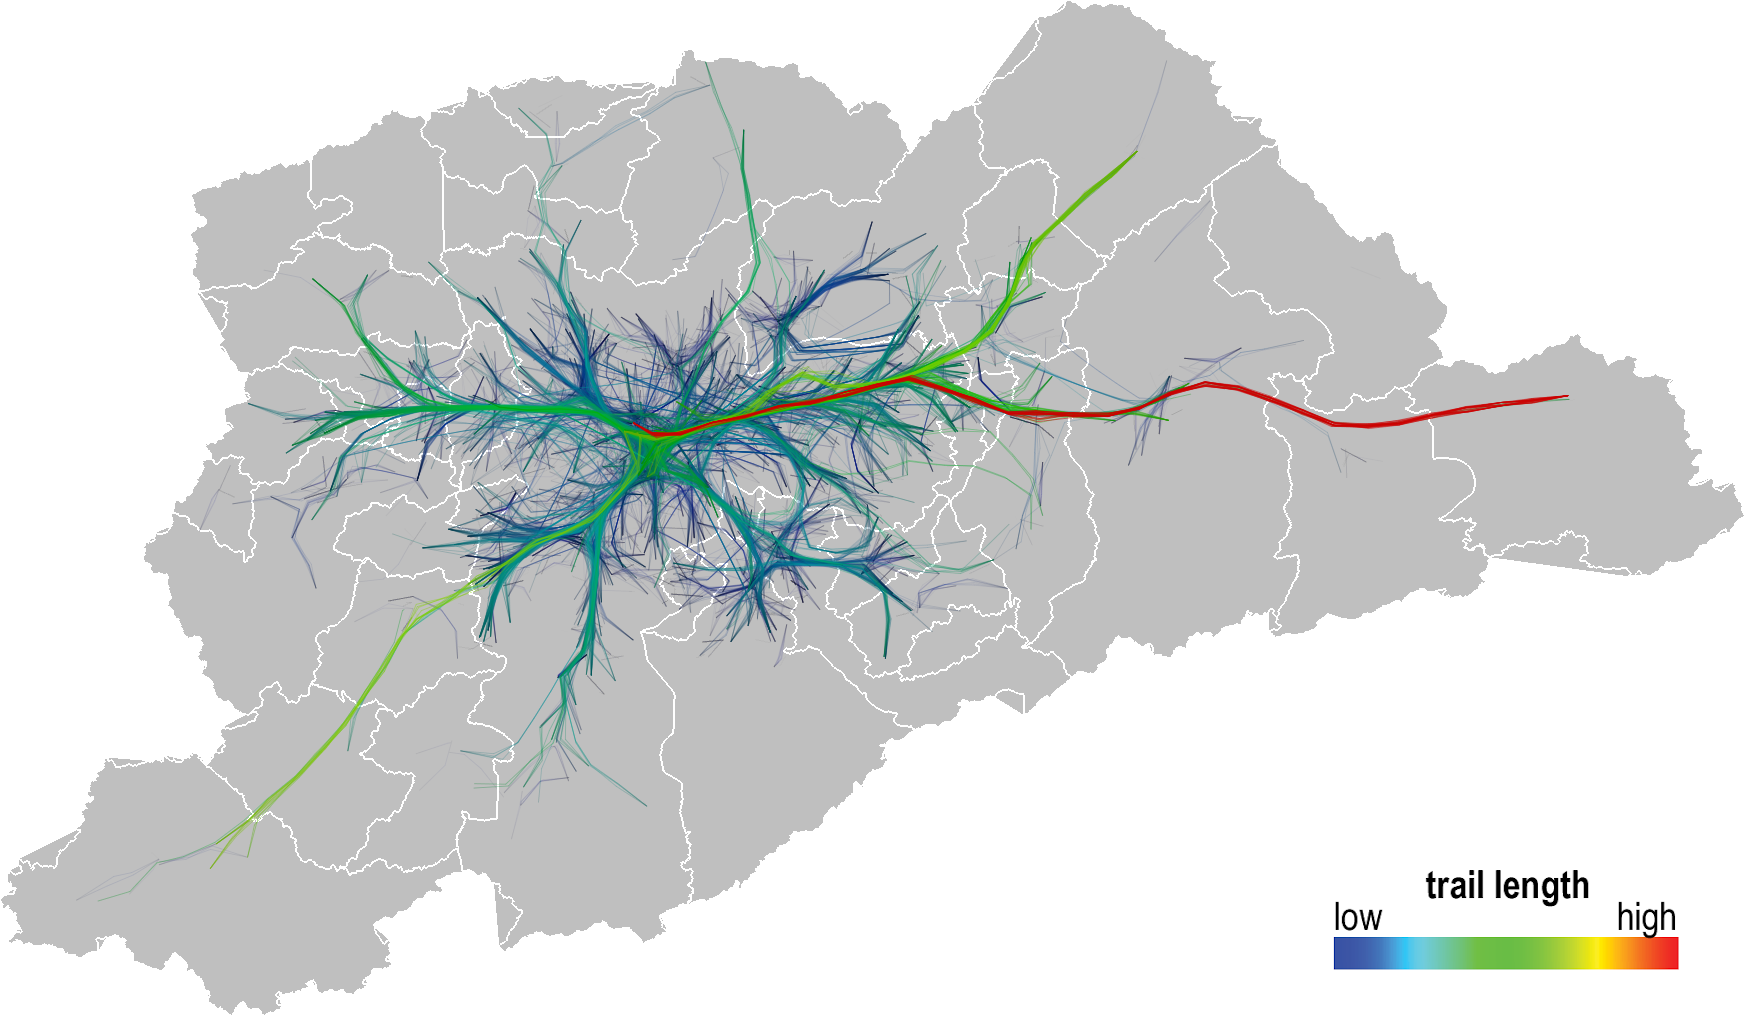
\includegraphics[width=0.98\textwidth]{../figuras/reason-health-leg.png}
\caption{Distâncias das viagens por motivo de saúde.\label{fig:reason-health}}
\end{figure}

\begin{figure}[!htb]
\centering
\captionsetup{justification=centering}
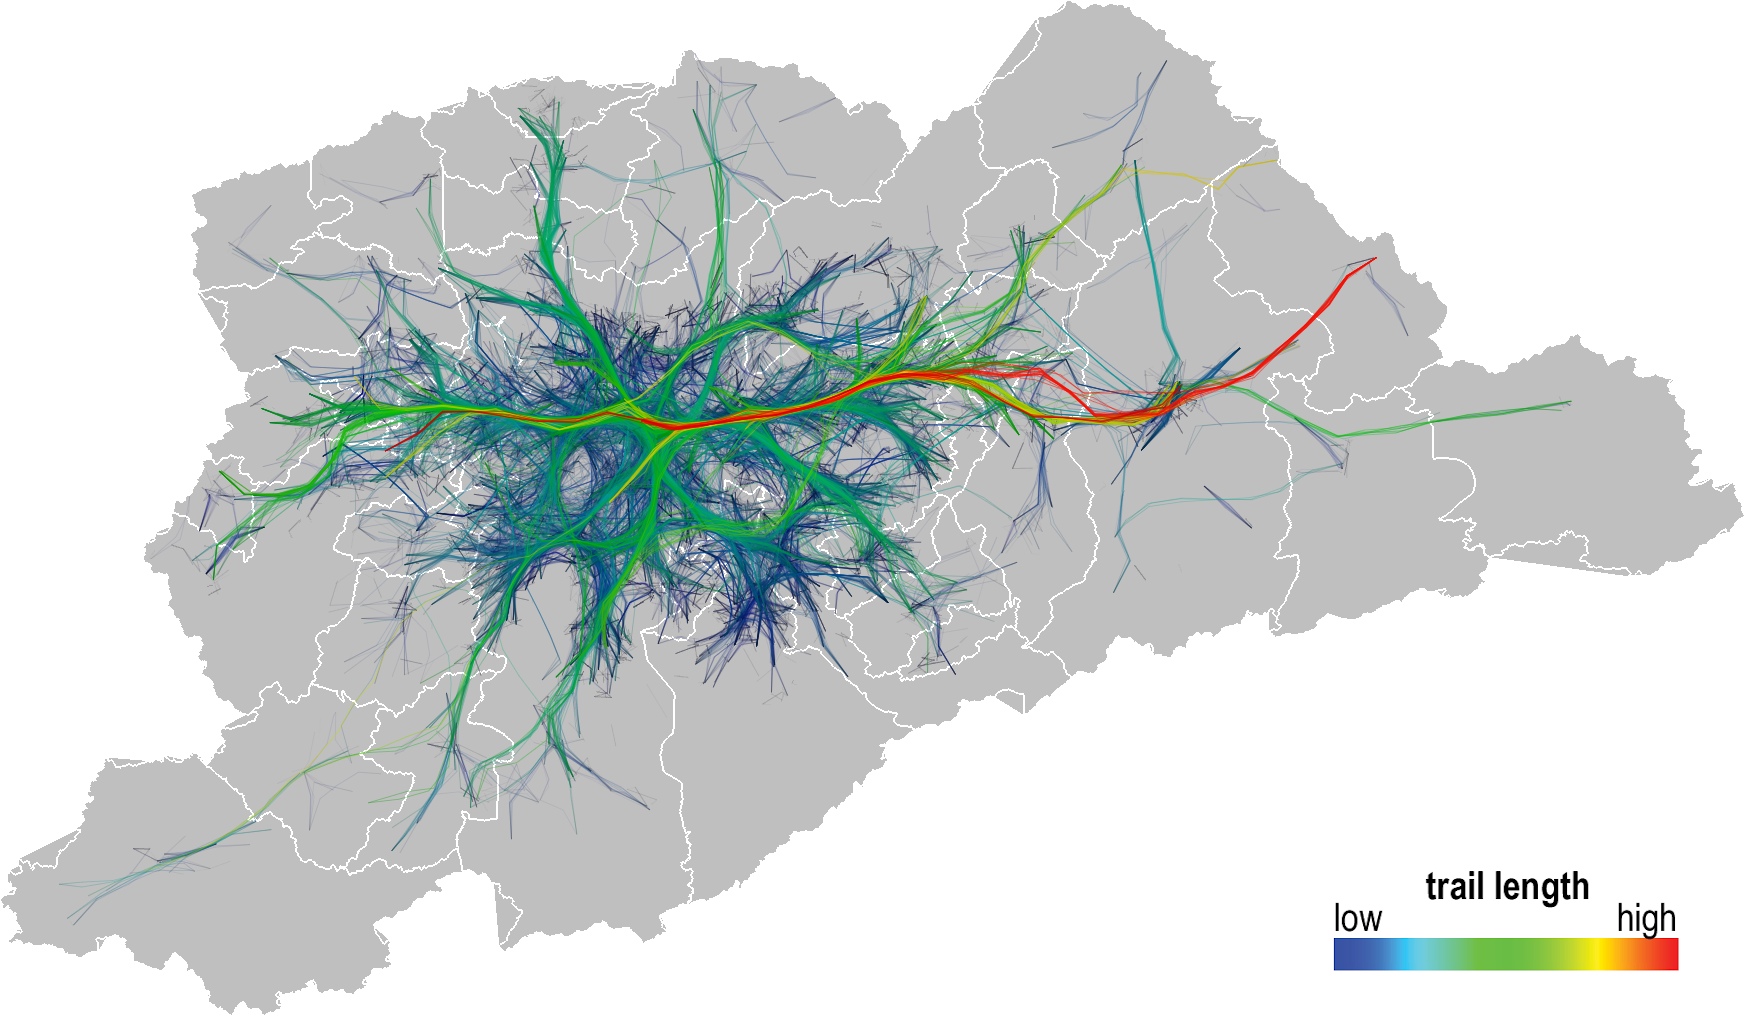
\includegraphics[width=0.98\textwidth]{../figuras/reason-school-leg.png}
\caption{Distâncias das viagens por motivo educação.\label{fig:reason-education}}
\end{figure}

\begin{figure}[!htb]
\centering
\captionsetup{justification=centering}
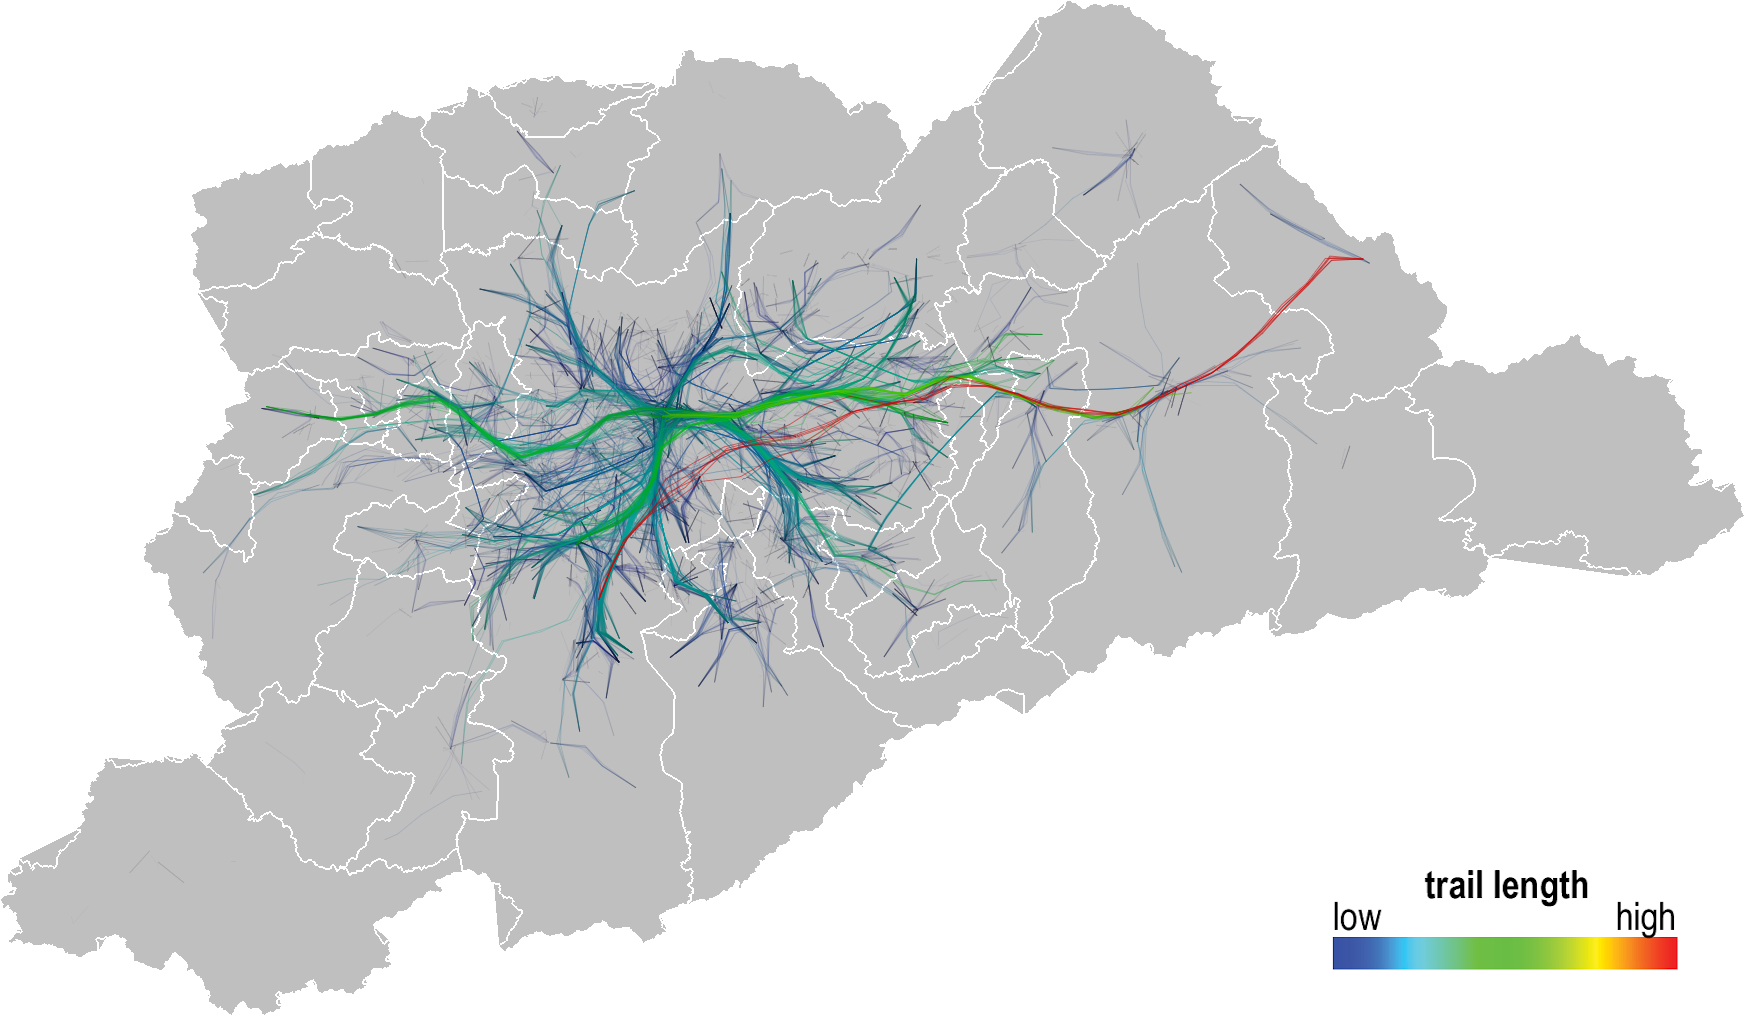
\includegraphics[width=0.98\textwidth]{../figuras/reason-shopping-leg.png}
\caption{Distâncias das viagens por motivo compras.\label{fig:reason-shopping}}
\end{figure}

